\documentclass[a4paper,fleqn]{cas-sc}

\usepackage[numbers,sort&compress]{natbib}
\usepackage[T1]{fontenc}
\usepackage{amsmath, amssymb}
\usepackage{booktabs}
\usepackage{multirow}
\usepackage{graphicx}

\begin{document}
\let\WriteBookmarks\relax
\def\floatpagepagefraction{1}
\def\textpagefraction{.001}

\shorttitle{Subject-Independent Detection of ADHD from Raw EEG: A Nested Cross-Validation Reassessment of CNN and Hybrid Classifiers}
\shortauthors{Abinaya G}

\title[mode=title]{Subject-Independent Detection of ADHD from Raw EEG: A Nested Cross-Validation Reassessment of CNN and Hybrid Classifiers}

\author[1]{Abinaya G}
\cormark[1]
\ead{abinaya.g05@gmail.com}

\affiliation[1]{organization={Saveetha Engineering College},
                city={Chennai},
                state={Tamil Nadu},
                country={India}}

\cortext[cor1]{Corresponding author}

\begin{abstract}
\textbf{Background.} Electroencephalography (EEG) is increasingly explored as a low-cost, non-invasive complement to behavioural assessment in attention-deficit/hyperactivity disorder (ADHD), and several studies applying convolutional neural networks (CNNs) directly to raw EEG have reported classification accuracies well above 90\%, occasionally approaching 100\%. A substantial share of this literature evaluates models by pooling short EEG segments (epochs) across subjects rather than by holding out entire subjects, which risks an optimistic bias when segments from the same child appear in both the training and the evaluation partition. \textbf{Objective.} We re-evaluated a CNN and hybrid-classifier pipeline originally developed for raw-EEG ADHD detection under a nested, subject-independent cross-validation design, and compared it against three established EEG deep-learning architectures (EEGNet, ShallowConvNet, DeepConvNet), a covariance-alignment domain-adaptation step (CORAL), and a sensitivity analysis of the assumed EEG sampling rate. \textbf{Methods.} We used a public 19-channel EEG dataset of 121 children (61 with ADHD, 60 typically developing controls; 508 thirty-second epochs) recorded during a visual attention task. Models were evaluated with 5 outer folds $\times$ 4 inner folds $\times$ 5 repetitions of subject-grouped cross-validation, in which the inner loop alone controlled early stopping and the outer-test subjects never contributed to any training, validation, or model-selection step. Epoch-level predictions were aggregated to one prediction per child (primary aggregation: mean predicted probability) before computing accuracy, balanced accuracy, sensitivity, specificity, precision, F1, Matthews correlation coefficient (MCC), and the area under the receiver operating characteristic curve (AUC). Ninety-five percent confidence intervals were obtained by subject-level bootstrap (2000 resamples). Pairwise model comparisons at the native resolution used a subject-level paired bootstrap and permutation test (one paired observation per subject, n = 121) with Holm--Bonferroni correction, rather than treating repeated cross-validation folds as independent observations; the resolution-sensitivity comparison (Section 4.8), whose 5 outer folds are not reused across repetitions, used a paired Wilcoxon signed-rank test with Holm--Bonferroni correction. \textbf{Results.} At the subject level, EEGNet achieved the highest balanced accuracy (0.793, 95\% CI 0.723--0.862; AUC 0.902, 95\% CI 0.844--0.949). Using a subject-level paired bootstrap and permutation test (n = 121 subjects, Holm-corrected within an 11-comparison family; Section 3.17), EEGNet, ShallowConvNet (balanced accuracy 0.737, 95\% CI 0.660--0.811), and the CNN-plus-logistic-regression classifier (balanced accuracy 0.743, 95\% CI 0.667--0.816) showed a statistically significant balanced-accuracy advantage over the plain CNN (balanced accuracy 0.547, 95\% CI 0.459--0.627). The remaining CNN-derived hybrid classifiers (radial-basis-function and linear support vector machines, random forest, k-nearest neighbours, Gaussian naive Bayes), and DeepConvNet, showed no statistically significant difference from the plain CNN under this test, despite several showing a higher point estimate. Covariance alignment (CORAL) applied to the logistic-regression classifier did not improve balanced accuracy relative to the unaligned classifier (0.735 versus 0.743). A sensitivity analysis comparing the native, assumed 128 Hz representation against a 128-to-512 Hz FFT-interpolated representation found no statistically significant difference for either CNN or EEGNet (both p > 0.18; 5 paired outer folds each); we do not interpret this as evidence about the recording's true sampling rate. \textbf{Conclusion.} Under subject-independent evaluation, this raw-EEG CNN/hybrid pipeline generalizes across held-out children in the 0.55--0.79 balanced-accuracy range depending on the classifier used, well below the near-ceiling figures reported by several recent segment-evaluated studies on related or identical data. The results support hybrid CNN-plus-classical-classifier and standard deep architectures (EEGNet in particular) as more promising directions than the plain CNN evaluated in the original study, while underscoring that subject-level, uncertainty-quantified evaluation is necessary before EEG-based ADHD classifiers can be meaningfully compared across studies or considered for any downstream clinical use.
\end{abstract}

\begin{keywords}
ADHD \sep  electroencephalography \sep  convolutional neural network \sep  subject-independent cross-validation \sep  nested cross-validation \sep  EEGNet \sep  domain adaptation \sep  CORAL
\end{keywords}

\maketitle

\section{Introduction}

Attention-deficit/hyperactivity disorder (ADHD) is one of the most commonly diagnosed neurodevelopmental conditions in childhood, with pooled worldwide prevalence estimates around 5\% in systematic reviews of the epidemiological literature \cite{polanczyk2007worldwide}. It is characterized by persistent, developmentally inappropriate patterns of inattention, hyperactivity, and impulsivity, and carries a substantial burden across academic, social, and family functioning that typically persists, in some form, well beyond childhood \cite{thapar2016attention,faraone2015attention}. Diagnosis currently rests on behavioural interviews, rating scales, and clinical judgement, all of which are informative but subjective, time-consuming, and dependent on the reporting accuracy of parents, teachers, and the children themselves. This has motivated a long-running search for objective, physiologically grounded measures that could complement --- not replace --- behavioural assessment. Electroencephalography (EEG) is an attractive candidate for this role: it is non-invasive, comparatively inexpensive relative to neuroimaging modalities such as fMRI, tolerates the fidgeting and short attention spans typical of the population being assessed, and has a decades-long history of association with ADHD through band-power and theta/beta-ratio findings --- most prominently an elevated theta/beta power ratio, reported in an early meta-analysis with a large pooled effect size \cite{snyder2006metaanalysis} but later shown to decline in reliability across the intervening decade of replication studies as control groups' own theta/beta ratios shifted over time \cite{arns2013decade}, to the point that a dedicated clinical-utility review concluded no single EEG measure, theta/beta ratio included, is yet suitable as a standalone diagnostic marker for ADHD \cite{loo2012clinical}. This inconsistency in the classical, hand-engineered EEG-marker literature is itself part of the motivation for the shift toward end-to-end deep learning discussed next: if a single, decades-studied spectral feature cannot reliably separate the two groups, a learned representation might succeed where a fixed one has not --- but only if that learned representation is evaluated in a way that actually tests generalization to new children, which is the central methodological question this paper investigates.



The last decade has seen a shift away from hand-engineered EEG features (band powers, connectivity metrics, entropy measures) toward end-to-end deep learning applied directly to raw or minimally processed EEG, mirroring a broader move in machine learning toward representation learning rather than fixed feature engineering \cite{lecun2015deep}. Two systematic reviews of this shift as it applies specifically to EEG decoding \cite{craik2019deep,roy2019deep} both note the same pattern that motivates the present study: reported classification performance varies enormously across papers using superficially similar deep architectures, and validation methodology --- not architecture alone --- is a major, often under-reported, source of that variance. Architectures such as EEGNet \cite{lawhern2018eegnet} and the Shallow/DeepConvNet family \cite{schirrmeister2017deep} were explicitly designed to let convolutional filters discover their own spatial and temporal patterns rather than relying on a predefined feature set, building on generic deep-learning components --- batch normalization \cite{ioffe2015batch}, dropout regularization \cite{srivastava2014dropout}, and gradient-based optimizers such as Adam \cite{kingma2015adam} --- that have become standard across the field since their introduction, and have since been adopted well beyond their original brain--computer-interface setting, including in ADHD classification. Within this trend, TaghiBeyglou et al. \cite{taghibeyglou2022detection} proposed a CNN architecture applied directly to raw, 19-channel EEG recorded from 61 children with ADHD and 60 typically developing controls, and additionally trained several classical classifiers (logistic regression, support vector machines, random forest, Gaussian naive Bayes, k-nearest neighbours) on the features extracted by the trained CNN's penultimate layer --- a hybrid design intended to combine the CNN's automatically learned representation with the different inductive biases of classical classifiers. That study, together with a large and rapidly growing surrounding literature reviewed in Section 2, reported pooled classification accuracies in the range of roughly 60--70\% for grouped, subject-aware ten-fold validation, alongside considerably higher --- in several recent cases, near-ceiling --- figures under other validation schemes \cite{amini2025adhdeepnet,hassan2024convolutional,esas2023detection,chen2019deep,latifi2024siamese,kasim2023identification,cura2024detection,bansal2025eeg,mao2025advanced,kim2025electroencephalogram}, a pattern that recurs across many EEG-ADHD papers and motivates the present study.



A methodological problem runs through a large part of this literature, and it is not specific to ADHD-EEG research: most raw-EEG recordings are split into many short, overlapping or non-overlapping segments ("epochs") before being fed to a classifier, because a single continuous recording per subject would otherwise provide far too few training examples for a deep network. If these epochs are then randomly assigned to training and test partitions without constraining all epochs from the same subject to the same partition, epochs from one child can appear on both sides of the split. Because consecutive or same-session EEG segments from one person share person-specific characteristics --- skull geometry, electrode-contact idiosyncrasies, baseline spectral tendencies, and, for a raw-signal CNN, potentially even amplifier or recording-session artefacts --- a classifier can partly learn to recognize the \textit{person}, not necessarily the \textit{condition}, and still score well on a test set that is not actually independent of the training set. This effect has been documented outside the EEG-ADHD literature in general terms: record-wise cross-validation has been shown to substantially overestimate accuracy relative to subject-wise cross-validation on the same data and models \cite{saeb2017need}, cross-validation used both for model selection and for the accuracy estimate produces an optimistically biased estimate of the true error unless a nested design is used \cite{varma2006bias}, and standard k-fold cross-validation has been shown, in simulation, to produce biased performance estimates at the sample sizes typical of clinical neuroimaging and EEG studies, whereas nested cross-validation and held-out test sets remain approximately unbiased regardless of sample size \cite{vabalas2019machine}. Whether, and to what extent, this same effect is present in a specific ADHD-EEG pipeline is an empirical question that can only be answered by re-running that pipeline under both validation regimes on the same data --- which is the starting point of the present study.



A second, related problem is architectural versus validation confounding. When two studies report different accuracies for two different EEG architectures on two different validation protocols, it is not possible to know whether the accuracy gap reflects the architectures or the protocols. Comparing CNN, EEGNet, ShallowConvNet, and DeepConvNet under one held constant, carefully controlled validation design --- rather than comparing each architecture's own reported number against a different architecture's own reported number under whatever protocol its authors chose --- is the only way to isolate an architectural effect from a validation effect.



A third issue, more specific to this particular dataset, concerns the assumed EEG sampling rate. The released recordings carry no explicit sampling-rate metadata; the widely used assumption of 128 Hz is inferred, not measured, from file duration and channel count. Because the original acquisition device is described elsewhere in the literature as capable of 512 Hz operation, several downstream reanalyses have quietly assumed the data could be treated as 512 Hz, or have upsampled it to 512 Hz, without being able to verify that no genuine 512 Hz content is being manufactured by interpolation. This is a preprocessing assumption worth testing explicitly rather than propagating silently.



This study addresses these three issues directly, using the same public dataset and the same core CNN/hybrid-classifier design as TaghiBeyglou et al. \cite{taghibeyglou2022detection}, but replacing the outer evaluation loop with a nested, nested-and-repeated, subject-grouped cross-validation design in which no epoch from an outer-test subject is ever used, in any capacity, before that subject's held-out prediction is made. We report results at the level of the child (the clinically relevant unit), not the epoch, and we quantify the resulting uncertainty with subject-level bootstrap confidence intervals rather than a single point estimate.



The contributions of this study are:



\begin{enumerate}

\item A leakage-controlled reimplementation of the CNN-and-hybrid-classifier ADHD-EEG pipeline, using nested, repeated, subject-grouped cross-validation (5 outer folds, 4 inner folds, 5 repetitions with independent seeds) in which the inner loop alone governs early stopping and the outer-test partition never contributes to model fitting, feature extraction, or classifier training in any fold.

\item A subject-level evaluation protocol --- aggregating epoch-level predictions to one prediction per child before computing performance --- reported alongside, and clearly distinguished from, the epoch-level pooled figures that dominate much of the surrounding literature.

\item A head-to-head comparison, under this identical protocol, of the original CNN, six CNN-derived classical classifiers, and three established EEG deep-learning architectures (EEGNet, ShallowConvNet, DeepConvNet), with subject-level bootstrap confidence intervals and Holm-corrected paired significance tests for every comparison.

\item A controlled evaluation of CORAL covariance alignment \cite{sun2016return} as a transductive, unsupervised domain-adaptation step between the outer-training and outer-test feature distributions, reporting covariance distance before and after alignment together with the resulting classifier performance.

\item An explicit sensitivity analysis of the assumed 128 Hz sampling rate, comparing native 128 Hz against FFT-interpolated 128-to-512 Hz representations under the same paired, subject-independent design, with the resampling procedure and its limitations stated plainly rather than described as a genuine higher-resolution acquisition.

\item A fully automated, 14-point structural and empirical leakage audit run on every experimental configuration, verifying --- rather than merely asserting from the presence of a grouped splitter --- that outer-test subjects never influence training, feature extraction, classifier fitting, early stopping, or normalization at any stage of the pipeline.

\end{enumerate}

The remainder of this paper is organized as follows. Section 2 reviews the ADHD-EEG classification literature, with particular attention to validation methodology and to how recently published studies on closely related or identical data report their performance. Section 3 describes the dataset, preprocessing, architectures, and evaluation protocol in full reproducible detail. Section 4 reports the results: dataset characteristics, the leakage audit, subject-level performance across all models, statistical comparisons, the CORAL analysis, and the resolution sensitivity analysis. Section 5 discusses these findings in relation to the literature reviewed in Section 2. Section 6 states the limitations of this study explicitly, and Section 7 concludes.



\section{Related Work}

\subsection{The dataset and the study being reassessed}

The dataset used throughout this paper --- 19-channel EEG from 61 children with ADHD and 60 typically developing controls, recorded during a visual attention task in which participants counted cartoon characters presented on screen --- was introduced by TaghiBeyglou et al. \cite{taghibeyglou2022detection}, who also proposed the CNN-plus-classical-classifier pipeline that this study re-evaluates. Their design trains a compact CNN directly on raw, per-epoch, per-channel-normalized EEG, then reuses the trained network's penultimate dense layer as a fixed feature extractor for logistic regression, a radial-basis-function support vector machine, a linear support vector machine, random forest, Gaussian naive Bayes, and k-nearest neighbours. Under grouped ten-fold cross-validation, they reported pooled accuracies in roughly the 60--70\% range for the plain CNN and several of its hybrid variants, a range broadly consistent with the epoch-level numbers we obtain under a considerably more conservative protocol (Section 4.3), even though our own subject-level, nested-cross-validation figures differ from any single pooled number their design produces, for the reasons discussed in Section 5.8.



\subsection{Deep learning architectures for raw EEG}

EEGNet \cite{lawhern2018eegnet} popularized a compact, depthwise-and-separable-convolution design intended to generalize across several brain--computer-interface paradigms (P300, error-related negativity, movement-related cortical potentials, sensory-motor rhythms) with a single, small architecture rather than a paradigm-specific one. ShallowConvNet and DeepConvNet, introduced together by Schirrmeister et al. \cite{schirrmeister2017deep}, instead pursue two points on a depth spectrum: a shallow, band-power-inspired design using a squaring nonlinearity and log-pooling loosely analogous to filter-bank common spatial patterns, and a deeper, four-block architecture intended to let the network learn a wider hierarchy of temporal-spatial features. Both papers report decoding accuracies competitive with or exceeding classical filter-bank baselines on motor and cognitive EEG decoding tasks, and both architectures have since been reused, adapted, or cited as baselines across a wide range of subsequent EEG classification studies, including several of the ADHD-specific studies discussed below. We implement all three networks in this study (Section 3) following their published architecture descriptions, rather than importing an external EEG-modelling package.



\subsection{Recent ADHD-EEG classification literature}

The pace of publication on EEG-based ADHD classification has increased substantially in the last three years, and a recent systematic review covering studies published between 2016 and 2022 catalogued a large and heterogeneous body of work spanning both MRI- and EEG-based approaches, machine learning and deep learning models, and a wide range of validation protocols, concluding that methodological diversity --- including inconsistent handling of subject-level partitioning --- remains a barrier to comparing reported performance figures across studies \cite{lohani2025systematic}. Individual studies published since that review's coverage window illustrate the same pattern. Esas and Latifoğlu \cite{esas2023detection} combined EEG sub-band decomposition (robust local mode decomposition and variational mode decomposition) with a custom deep-learning classifier on 19-channel EEG, reporting over 95\% accuracy for ADHD-versus-control discrimination. Hassan and Singhal \cite{hassan2024convolutional} proposed a two-convolutional-layer CNN trained on band-pass-filtered, 5-second EEG segments and reported 100\% accuracy, sensitivity, and specificity using the full 19-channel montage, with only a modest drop (99.08\% accuracy) when restricted to frontal channels alone. Most directly relevant to the present study, Amini et al. \cite{amini2025adhdeepnet} introduced ADHDeepNet, a temporal-spatial CNN with an adaptive squeeze-and-excitation attention mechanism and an integrated-gradients-based explainability component, evaluated --- by the authors' own description --- with nested cross-validation on the same 121-participant (61 ADHD, 60 control) dataset used here, and reported 99.17\% accuracy with 100\% sensitivity. A more recent multiscale convolutional architecture, EEG-MSCNet, evaluated with subject-level leave-one-subject-out validation on a related pediatric EEG dataset, reported a substantially more modest 87.6\% accuracy and 88.2\% AUROC \cite{sanchis2026multiscale} --- a figure much closer to the subject-level results obtained in the present study (Section 4) than the near-ceiling accuracies reported elsewhere in this literature.



This pattern extends well beyond the four studies discussed above. Chen, Song, and Li \cite{chen2019deep} proposed one of the earlier deep-learning approaches to this problem, combining a mutual-information-based EEG brain network with a CNN on a separate 50-ADHD/51-control cohort. Latifi, Amini, and Motie Nasrabadi \cite{latifi2024siamese} --- overlapping in authorship with the ADHDeepNet study \cite{amini2025adhdeepnet} --- applied a Siamese convolutional network to power-spectral-density brain maps derived from what appears to be the same underlying dataset used throughout the present paper, again reporting 99.17\% accuracy, and used Grad-CAM attribution to highlight frontal and occipital theta-band features as the model's primary discriminators. Kasim \cite{kasim2023identification} combined multitaper and multivariate variational mode decomposition with a convolutional-recurrent hybrid network, and Karabiber Cura, Akan, and Kocaaslan \cite{cura2024detection} constructed image-like EEG feature maps as CNN input, both on separately sourced cohorts. Bansal, Gangwar, Aljaidi, Alkoradees, and Singh \cite{bansal2025eeg} combined autoencoder feature extraction with a ResNet-style architecture and a double attention mechanism; Mao, Qi, He, Wang, Wang, and Wang \cite{mao2025advanced} took a more classically grounded route, extracting power-spectral-density, fuzzy-entropy, and mutual-information connectivity features and using SHAP-based feature selection ahead of a machine-learning classifier rather than an end-to-end deep network; and Kim, Kim, Kim, Yang, and Kwon \cite{kim2025electroencephalogram}, working with a larger, independently collected 168-participant sample (107 ADHD, 61 control), trained gradient-boosted classifiers on band-power features across five frequency bands and again used SHAP values to identify contributing features, reporting accuracy in a considerably more modest range consistent with the classical band-power literature discussed above \cite{snyder2006metaanalysis,arns2013decade,loo2012clinical} than with the near-ceiling figures reported by several of the raw-EEG deep-learning studies. A further, closely related architecture search line --- the recently updated systematic review \cite{lohani2025systematic} --- catalogues dozens of further examples with comparably heterogeneous validation protocols.



This spread --- from EEG-MSCNet's 87.6\% under leave-one-subject-out validation, to Kim et al.'s more modest gradient-boosted-feature figures on an independent cohort \cite{kim2025electroencephalogram}, to several other studies' 95--100\% under designs described only briefly in their respective publications \cite{amini2025adhdeepnet,hassan2024convolutional,esas2023detection,chen2019deep,latifi2024siamese} --- is difficult to interpret without full visibility into how each study assigned segments to folds, whether early stopping or hyperparameter selection ever had access to test-fold subjects, and whether performance was computed per segment or per participant. We do not have access to the training code or fold assignments of Amini et al. \cite{amini2025adhdeepnet}, Hassan and Singhal \cite{hassan2024convolutional}, or Latifi et al. \cite{latifi2024siamese}, and we are consequently not in a position to state that any of these studies' specific pipelines contain subject leakage; we can state only that a 99--100\% classification accuracy for a binary, clinically defined condition from 19-channel EEG in a sample of this size is, on prior grounds, an unusual result relative to the diagnostic accuracy of most single-modality physiological biomarkers in psychiatry, and that our own subject-level, nested-cross-validation results on directly comparable --- in the case of Amini et al. and Latifi et al., apparently the same --- data fall far short of it (Section 5.8). This gap is the central empirical motivation for reporting validation methodology in as much explicit, checkable detail as Section 3 attempts to provide.



\subsection{Cross-subject generalization and domain adaptation in EEG decoding}

The difficulty of generalizing an EEG classifier from a set of training subjects to unseen subjects is a recognized problem well beyond ADHD classification, arising from substantial inter-subject variability in skull and cortical anatomy, electrode contact, and idiosyncratic neural dynamics. A recent survey organizes the deep-learning methods proposed to address this cross-subject domain shift into feature-alignment, adversarial-learning, feature-disentanglement, and contrastive-learning families, and identifies the treatment of subject identity as a structural, rather than incidental, modelling choice for future EEG decoding systems \cite{li2026crosssubject}. CORAL --- correlation alignment --- is one of the earliest and simplest members of the feature-alignment family: it aligns the second-order statistics (covariance) of a source and a target feature distribution via a closed-form whitening-and-recoloring transform, requiring no target labels and no iterative optimization \cite{sun2016return}. It has since been extended into a differentiable "Deep CORAL" loss for end-to-end training and applied within EEG motor-imagery decoding pipelines that combine deep feature extraction with an explicit correlation-alignment loss to reduce cross-subject or cross-session distribution shift \cite{zhong2023deep}. The present study applies the original, non-deep CORAL formulation to the fixed features extracted by a trained CNN, aligning the outer-test subjects' unlabelled feature covariance toward the outer-training subjects' covariance, and reports this explicitly as a transductive, unsupervised setting rather than as an inductive subject-independent evaluation (Section 3.18), following the same logic used to characterize domain-adaptation experiments in the broader EEG transfer-learning literature.



\subsection{Explainability}

Integrated Gradients \cite{sundararajan2017axiomatic} attributes a deep network's prediction to its input features by integrating the gradient of the output with respect to the input along a straight-line path from a baseline (typically an all-zero input) to the actual input, satisfying axioms --- sensitivity and implementation invariance --- that several earlier gradient-based attribution methods do not. It has been adopted in several recent EEG-ADHD studies, including ADHDeepNet \cite{amini2025adhdeepnet}, as a means of visualizing which channels and time windows most influence a trained network's decision. In the present study we compute Integrated Gradients attributions as a supplementary, visualization-only analysis (Section 3.19) and do not treat the resulting channel and temporal importance maps as evidence of classification performance or of any causal neurophysiological claim.



\subsection{Methodological literature on cross-validation bias}

The statistical case for the validation design adopted here is not specific to EEG. Varma and Simon \cite{varma2006bias} showed formally and empirically that using cross-validation both to select a model (or its hyperparameters) and to estimate that model's error produces an optimistically biased error estimate, and that a nested cross-validation design --- an inner loop for selection, an outer loop for evaluation, with the outer-test data touching only the evaluation step --- removes this bias. Saeb et al. \cite{saeb2017need}, working in a mobile-health rather than an EEG setting, demonstrated directly that record-wise cross-validation (analogous to epoch-wise cross-validation in EEG) can report an error rate that changes little as the number of folds increases, while the corresponding subject-wise cross-validation error changes substantially, illustrating that a low record-wise error need not reflect the accuracy a deployed, subject-independent system would actually achieve. Vabalas et al. \cite{vabalas2019machine} extended this line of evidence with simulation studies spanning a range of sample sizes broadly comparable to those seen in clinical EEG and neuroimaging research, showing that ordinary k-fold cross-validation remains biased even as the sample size grows into the low thousands, whereas nested cross-validation and held-out test sets do not. Together, these three studies form the direct methodological basis for the nested, repeated, subject-grouped design adopted in Section 3, and for treating the paired, per-outer-fold subject-level estimate --- rather than a single pooled number --- as the correct unit of statistical comparison between models (Section 3.17).



\section{Materials and Methods}

\subsection{Dataset}

We used the public 19-channel EEG dataset introduced by TaghiBeyglou et al. \cite{taghibeyglou2022detection}, comprising 121 children: 61 diagnosed with ADHD and 60 typically developing controls, recorded during a visual attention task in which each child was shown a sequence of cartoon images and asked to count the number of characters depicted. Electrodes were placed according to the international 10--20 system. The released files contain no explicit sampling-rate metadata; a rate of 128 Hz is assumed throughout this study, consistent with the assumption made in the original study, and inferred from file duration relative to the 30-second epoch length used for segmentation rather than measured directly. This assumption, and its consequences, are examined explicitly in Section 3.19 and Section 4.8 rather than treated as an established fact.



\subsection{EEG acquisition and task}

Recordings were collected during a sustained visual-attention paradigm (cartoon-character counting) rather than a resting-state protocol, meaning the classification target reflects EEG activity during active, sustained attentional engagement rather than an unconstrained resting state. We did not have access to trial-by-trial behavioural performance (e.g., counting accuracy) alongside the EEG, and this study makes no claim about the relationship between task performance and the EEG-derived classification.



\subsection{Data organization and subject identification}

Each subject's continuous recording is stored as a separate file, and every epoch extracted from a given file is assigned that file's identifier as its subject ID. Subject identity is therefore determined structurally by data provenance rather than by any label inferred from the EEG itself, which is a precondition for the grouped cross-validation described in Section 3.12: as long as subject ID is correctly propagated (verified in Section 4.2), a subject-grouped split cannot accidentally split one child's epochs across two folds.



\subsection{Preprocessing}

Each 30-second segment ("epoch") is normalized independently, per channel, by subtracting that epoch's own per-channel mean and dividing by that epoch's own per-channel standard deviation (a per-epoch z-score). Because this normalization statistic is computed exclusively from the epoch being normalized, it cannot depend on, or leak information from, any other epoch --- including any epoch belonging to a different (e.g., outer-test) subject --- regardless of how the data are later partitioned into folds. No filtering, artifact rejection, or channel selection beyond what is described here was applied; the goal of this study is to reassess the validation methodology applied to a raw-EEG pipeline, not to introduce a new preprocessing stream.



\subsection{Epoch segmentation}

Each subject's continuous recording is segmented into non-overlapping 30-second epochs at the assumed 128 Hz sampling rate, yielding 3840 samples per epoch across the 19 channels. This segmentation produced 508 epochs in total across the 121 subjects (288 from ADHD subjects, 220 from control subjects); because recording lengths vary across subjects, the number of epochs per subject is not constant, a fact that is directly relevant to why subject-level, rather than epoch-level, aggregation is used as the primary evaluation unit (Section 3.14).



\subsection{CNN architecture}

The CNN follows the architecture used in the original study \cite{taghibeyglou2022detection}: two spatial convolutional blocks (10$\times$1 and 4$\times$1 kernels across the channel dimension, each followed by batch normalization and average pooling) reduce the 19-channel input to a single spatial dimension, after which the representation is reshaped into a one-dimensional temporal sequence and passed through two temporal convolutional blocks whose kernel sizes scale with the assumed sampling rate (fs/4 and fs/8 samples respectively, so that the same architecture definition is reused, with different effective receptive fields, for both the native 128 Hz and the 512 Hz-interpolated sensitivity condition described in Section 3.19). The result is flattened and passed through two dense layers (64 and 32 units, ReLU activation) before a final sigmoid output unit. The 64-unit dense layer is also exposed as a separate feature-extraction output, used by every hybrid classifier described in Section 3.8.



\subsection{CNN-derived feature extraction}

For every outer fold, the 64-dimensional activation of the CNN's first dense layer, computed from the same CNN instance trained for that specific fold, is extracted for both the outer-training and outer-test epochs. These features --- never the raw EEG --- are what the classical classifiers in Section 3.8 are trained and evaluated on. Because a new CNN is trained independently for every outer fold (Section 3.12), the feature extractor used for any given fold's classical classifiers is always the one trained without access to that fold's outer-test subjects.



\subsection{Classical hybrid classifiers}

Six classical classifiers are trained on the CNN-derived features described above: logistic regression (L2-penalized, balanced class weights), a linear support vector machine (balanced class weights, probability outputs enabled), a radial-basis-function support vector machine (referred to throughout as NLSVM, for "non-linear SVM"; balanced class weights), a random forest (100 trees, balanced class weights), Gaussian naive Bayes, and a k-nearest-neighbours classifier (k = 5). Gaussian naive Bayes and k-nearest neighbours do not expose a class-weighting mechanism in the scikit-learn implementation used here and were therefore trained without class weighting; this is stated explicitly because it is a plausible partial explanation for these two classifiers' comparatively higher sensitivity and lower specificity relative to the balanced-class-weight classifiers (Section 4.3, Section 5.3). Every classifier is refit from scratch on each outer fold's training features and evaluated once on that fold's outer-test features.



\subsection{EEGNet}

We reimplemented EEGNet following the architecture described by Lawhern et al. \cite{lawhern2018eegnet}: an initial temporal convolution, a depthwise spatial convolution across the full channel dimension with a unit-norm weight constraint, batch normalization, an ELU nonlinearity, average pooling and dropout, followed by a separable convolution, a second average-pooling-and-dropout stage, and a final dense classification layer with a norm constraint. The temporal kernel length scales with the assumed sampling rate. As with the CNN, the 64-unit dense layer immediately before the output is also exposed as a feature-extraction output for architectural consistency with the rest of the pipeline, although the classical hybrid classifiers of Section 3.8 were applied only to CNN features, not to EEGNet, ShallowConvNet, or DeepConvNet features, in the experimental configuration reported here.



\subsection{ShallowConvNet}

ShallowConvNet was reimplemented following Schirrmeister et al. \cite{schirrmeister2017deep}: a temporal convolution followed by a spatial convolution across the channel dimension, batch normalization, a squaring nonlinearity, average pooling, a logarithmic nonlinearity, and dropout, before flattening into a dense classification layer. Kernel and pooling sizes scale with the assumed sampling rate, following the scaling ratios described in the original paper.



\subsection{DeepConvNet}

DeepConvNet was reimplemented following the same source \cite{schirrmeister2017deep}: an initial temporal-then-spatial convolutional block (25 filters) followed by three further convolutional blocks of increasing width (50, 100, and 200 filters), each with batch normalization, an ELU nonlinearity, max pooling, and dropout, before flattening into a dense classification layer.



\textit{A caveat applies to Sections 3.9--3.11 collectively}: EEGNet, ShallowConvNet, and DeepConvNet were reimplemented directly from the architecture descriptions published in \cite{lawhern2018eegnet} and \cite{schirrmeister2017deep}, because independent verification of the corresponding reference implementations against these descriptions, layer width by layer width and kernel size by kernel size, was not performed as part of this study. We report the exact layer configuration used (Sections 3.9--3.11 and the accompanying source code) so that any discrepancy from the original authors' own implementations can be identified and corrected, and we treat these three architectures in the Results and Discussion as close reimplementations following the published descriptions, not as verified exact reproductions.



\subsection{Nested subject-independent cross-validation}

The central methodological change relative to the original study \cite{taghibeyglou2022detection} is the replacement of a single grouped k-fold split with a nested, repeated design. For each of 5 repetitions (independently seeded, Section 3.13), the 121 subjects are partitioned into 5 outer folds using a class-balanced, seed-shuffled adaptation of group k-fold splitting: the unique subject list is shuffled under that repetition's seed, subjects are then distributed round-robin by diagnostic label across the 5 folds to keep each fold's ADHD/control ratio close to the overall dataset ratio, and the resulting fold assignment guarantees --- by construction --- that no subject is split across folds. For each outer fold, the remaining four folds' subjects form the outer-training set. Within that outer-training set only, a 4-fold group k-fold split (scikit-learn's \texttt{GroupKFold}) forms the inner loop: for each of the 4 inner folds, a fresh model is trained on the inner-training subjects with early stopping monitored on the inner-validation subjects' loss, and the training epoch at which that inner fold's monitored loss was minimized is recorded. The median of these four recorded epoch counts, across the four inner folds, is then used as a fixed training budget to fit one final model on \textit{all} of that outer fold's training subjects, without any validation split at all in this final fit --- meaning no early-stopping signal of any kind is available during this final fit, because the number of training epochs was already fixed by the inner loop before this fit began. This final model is then evaluated exactly once, on the outer-test subjects, who have not contributed an epoch to any step of the process described above --- not the inner splits, not the early-stopping decision, not the final fit, and, for the classifiers in Section 3.8, not the feature-extractor training either. Figure 1 shows this design schematically for one repetition's 5 outer folds.



\begin{figure}[htbp]

\centering

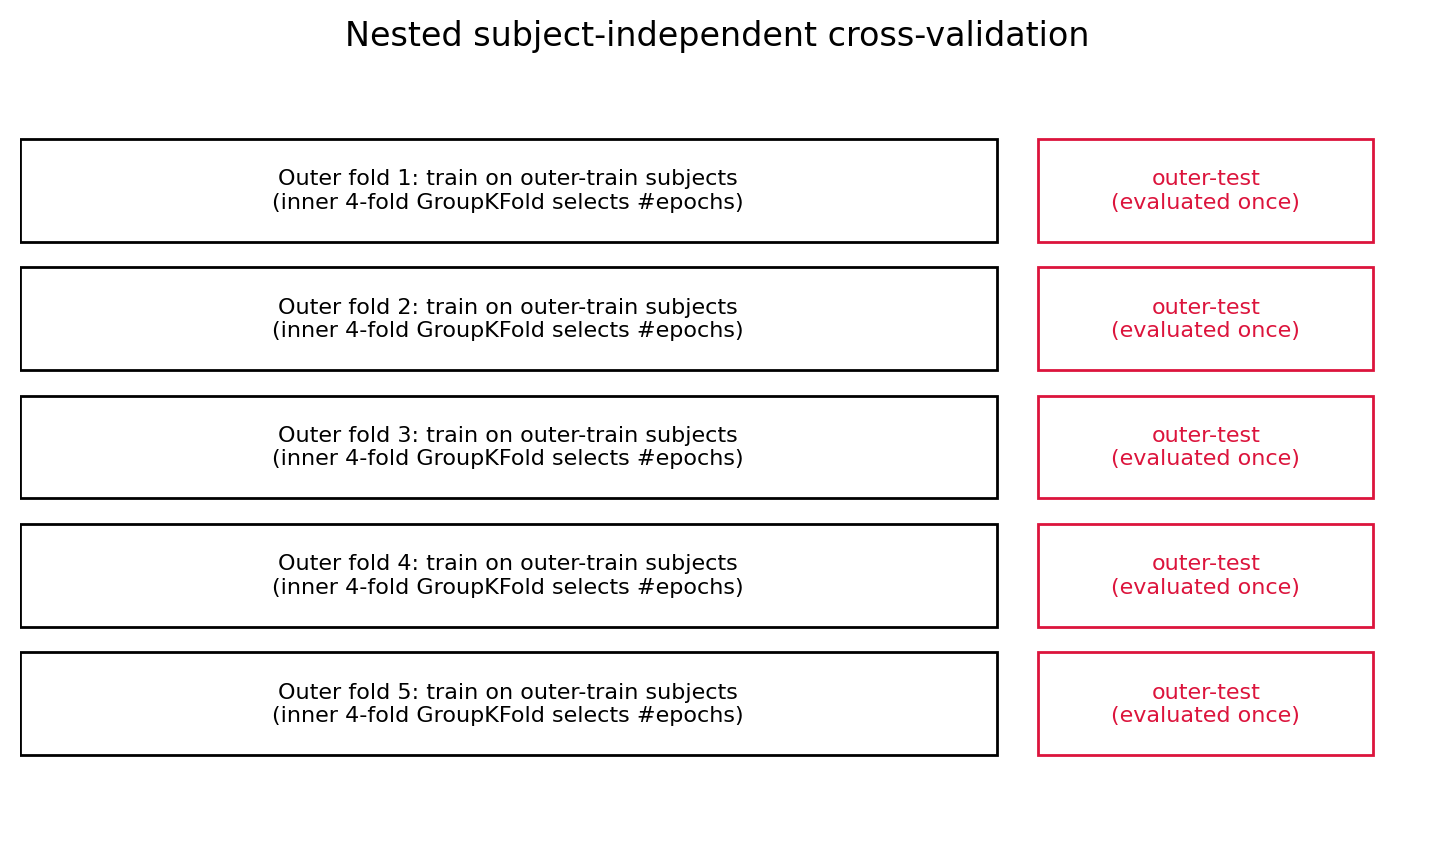
\includegraphics[width=\textwidth]{FIGURES/fig3_nested_cv_schematic.png}

\caption{Schematic of the nested, subject-grouped cross-validation design for one repetition (5 outer folds). Each outer fold trains on that fold's outer-train subjects, with an inner 4-fold GroupKFold split (not shown at this resolution) selecting the training-epoch budget; the outer-test subjects (right, red) are evaluated exactly once and never contribute to any training or selection step.}

\label{fig:1}

\end{figure}

\subsection{Repeated evaluation and random seeds}

The entire outer-fold procedure described in Section 3.12 is repeated five times with five independent seeds (42, 43, 44, 45, 46), each producing a different random shuffling of subjects into outer folds (and, within each outer fold, a different random shuffling into inner folds). Every model-fitting call is preceded by a call that seeds Python's own random-number generator, NumPy, and TensorFlow using a seed derived from the repetition and outer-fold index, so that a given fold's training is reproducible given the same code and the same hardware, with the documented exception that certain GPU convolution kernels retain a small amount of run-to-run nondeterminism even under a fixed seed; CPU execution is deterministic under these seeds. Five repetitions across five outer folds yield 25 outer-fold evaluations per model at the native 128 Hz condition --- the correct way to describe this quantity, adopted throughout this paper, is 25 \textit{paired outer-fold performance estimates drawn from five repeated five-fold partitions of the same 121 subjects}, not 25 independent subject cohorts, since the same subjects reappear, under a different partition, in every repetition.



\subsection{Subject-level aggregation}

Because the number of 30-second epochs per subject varies (Section 3.5), a classifier could in principle appear to perform well or poorly simply because of how many epochs a particular subject happens to contribute, if epoch-level predictions were treated as independent observations and pooled directly. We therefore treat the child, not the epoch, as the primary unit of analysis. For every outer-test subject, all of that subject's epoch-level predicted probabilities are averaged into a single subject-level probability (mean-probability aggregation), which is then thresholded at 0.5 to produce that subject's predicted label; this mean-probability aggregation is the primary aggregation method used for every headline result in Section 4. As a secondary, exploratory aggregation, we also computed a majority-vote label from each subject's epoch-level predicted labels; both aggregations are reported side by side in Table 3, and the two agree closely for most models and diverge somewhat for models with an epoch-level bias toward one class (Section 4.3).



\subsection{Performance metrics}

At the subject level, we report accuracy, balanced accuracy, sensitivity (recall for the ADHD class), specificity (recall for the control class), precision, F1-score, the Matthews correlation coefficient (MCC \cite{chicco2020advantages}, preferred here alongside the other metrics because it is computed from all four confusion-matrix cells and is less easily inflated by class imbalance than accuracy or F1 alone), and the area under the receiver operating characteristic curve (AUC, computed from the aggregated subject-level probability, not from a thresholded label). Balanced accuracy --- the mean of sensitivity and specificity --- is used as the primary metric for ranking and for statistical comparison throughout Section 4 and Section 5, because the dataset's class sizes (61 versus 60 subjects) are close to balanced but the same is not always true within a given outer-test fold, and because balanced accuracy is less sensitive than raw accuracy to a classifier's operating point on the sensitivity/specificity trade-off.



\subsection{Bootstrap confidence intervals}

Ninety-five percent confidence intervals for every subject-level metric were obtained by a subject-level, non-parametric bootstrap \cite{efron1979bootstrap}: for a given model and preprocessing condition, the pooled subject-level table (one row per subject, using that subject's mean-probability aggregation) was resampled with replacement 2000 times, the metric of interest was recomputed on each resample, and the interval reported is the 2.5th-to-97.5th percentile of the resulting bootstrap distribution. Resampling was performed over subjects, never over individual epochs, so that the reported uncertainty reflects sampling variability across children rather than the pseudo-replicated variability that would result from treating multiple epochs of the same child as independent bootstrap units.



\subsection{Statistical comparisons}

\textbf{Why the primary test is subject-level, not fold-level.} An earlier version of this analysis compared models using a Wilcoxon signed-rank test applied to 25 per-(repetition, outer-fold) balanced-accuracy values (5 repetitions $\times$ 5 outer folds). We do not use that procedure as the primary inferential test in this paper, because those 25 values are not 25 independent observations: every repetition reuses the same 121 subjects, merely reshuffled into a different fold partition, so a subject who is unusually easy or unusually hard to classify contributes correlated information to as many as 5 of the 25 values. Treating repeated-CV fold estimates as independent replicates in this way is a form of pseudo-replication that can understate the true sampling uncertainty and yield artificially small p-values; we return to this as a named limitation in Section 6.



\textbf{Primary procedure.} For each pairwise comparison, we instead construct exactly one paired observation per subject (n = 121): each model's per-subject prediction is the same mean-probability aggregation used for Table 3 and Table 4 (that subject's predicted probability pooled across all epochs and all 5 repetitions, thresholded at 0.5; Section 3.14), so every subject contributes a single paired data point regardless of how many folds or repetitions its epochs happened to fall into. We report two complementary resampling-based tests on this paired, subject-level data: (i) a paired bootstrap, in which the 121 subject indices are resampled with replacement 20,000 times, the same resampled indices are applied to both models' predictions to preserve the pairing, and both models' balanced accuracy is recomputed on each resample, yielding a bootstrap distribution of the balanced-accuracy difference, its mean, its 95\% percentile confidence interval, and a two-sided p-value (2 $\times$ min[P(diff $\leq$ 0), P(diff $\geq$ 0)], capped at 1, equivalent to inverting the percentile confidence interval); and (ii) a paired permutation test, in which, independently for each subject, the two models' predictions are swapped with probability 0.5 (testing the null hypothesis that which model produced a given subject's prediction is exchangeable), repeated 20,000 times, with a two-sided p-value computed as the proportion of permuted differences at least as extreme as the one observed. We report both because they rest on different assumptions and, where they agree, that agreement is itself informative; where they disagree, we report both values rather than the more favorable one. A bootstrap-based standardized effect size (the observed mean difference divided by the bootstrap standard deviation of that difference) is reported alongside each comparison.



All comparisons in Table 5 are made against the plain CNN at 128 Hz as the pre-specified reference model, restricted to the native 128 Hz condition (11 comparisons: every other model evaluated at 128 Hz); both the bootstrap and the permutation p-values are Holm--Bonferroni corrected \cite{holm1979simple} within that 11-comparison family. The 128-to-512 Hz interpolation condition (Table 6) concerns a different scientific question (resolution sensitivity, not model superiority at the native resolution) and is corrected within its own, separate, 2-comparison family; because the interpolation condition was run for a single repetition only (Section 3.19), its 5 outer folds are a genuinely disjoint, non-reused subject partition, so the pseudo-replication concern above does not apply there and the original per-fold Wilcoxon signed-rank test \cite{wilcoxon1945individual} is retained for Table 6. Consistent with standard practice, we do not treat a non-significant p-value as evidence of equivalence between two models or two conditions; we describe such results as "no statistically significant difference was detected" rather than as "no difference exists."



\subsection{CORAL domain adaptation}

For the outer-fold-specific CNN feature extractor described in Section 3.7, we additionally computed a CORAL-aligned version of the outer-training features: the outer-training (source) features are whitened by the inverse square root of their own covariance matrix and then re-colored by the square root of the outer-test (target) features' own covariance matrix, following the closed-form correlation-alignment procedure of Sun, Feng, and Saenko \cite{sun2016return}. Critically, the target covariance is computed from the outer-test subjects' \textit{unlabelled} features only --- no outer-test label is used anywhere in this computation --- but the outer-test features themselves are used to compute that covariance before the outer-test evaluation is performed, which makes this a transductive, unsupervised domain-adaptation setting, not a standard inductive subject-independent evaluation; we report it as such throughout, following the same convention used to describe comparable domain-adaptation evaluations elsewhere in the EEG literature \cite{li2026crosssubject,zhong2023deep}. Two logistic-regression classifiers are then trained per outer fold: one on the unaligned outer-training features, and one on the CORAL-aligned outer-training features, and both are evaluated on the same outer-test features. The covariance distance (Frobenius norm of the difference between the source and target covariance matrices) is computed both before and after alignment, so the magnitude of the alignment's effect can be reported quantitatively rather than assumed. We note as an internal-consistency check, not a methodological flaw, that the "without CORAL" logistic-regression classifier in this comparison is mathematically identical to the standalone CNN+LR classifier reported elsewhere in this paper --- both are an L2-penalized, class-balanced logistic regression fit on the same outer-training CNN features and evaluated on the same outer-test CNN features --- and the results in Table 2, Table 3, and Table 4 confirm this: the two configurations' metrics agree to at least six decimal places in every case, exactly as expected from two runs of a deterministic classifier on identical inputs. As specified in the study scope (Section 1), no additional CORAL variant, alternative alignment target, or alternative base classifier was introduced beyond this single, pre-specified comparison.



\subsection{Resolution sensitivity analysis}

Because the dataset's true sampling rate is not verifiable from the released files (Section 3.1), we tested whether the assumed 128 Hz representation and a higher-resolution representation of the same recordings yield different classification performance. The higher-resolution representation was produced by FFT-based polyphase interpolation (\texttt{scipy.signal.resample}) of each 128 Hz epoch up to an effective 512 Hz, using the same 30-second epoch boundaries and therefore 15,360 samples per epoch instead of 3840. This is \textbf{interpolation of the existing 128 Hz samples, not a reconstruction of a genuine 512 Hz acquisition}: it can smooth and resample the signal already present, but it cannot introduce any spectral content above the original 128 Hz recording's actual Nyquist frequency that was not already implicitly present in the 128 Hz samples, whatever that frequency in fact was. We use the term "128-to-512 Hz interpolation" throughout this paper specifically to avoid the impression, present in some downstream secondary analyses of this dataset, that this procedure reproduces a genuine higher-sampling-rate recording. Because training four additional deep architectures at four times the sequence length across the full 5-repetition design was judged computationally disproportionate to the scientific question being asked (whether resolution matters at all, not how it interacts with every architecture and every repetition), this sensitivity analysis was run for the plain CNN and for EEGNet only, using a single repetition (the same subject partition and seed as the first repetition of the primary 128 Hz design, so that the two conditions are validly paired per outer fold, as required by Section 3.17), with the CNN's temporal kernel sizes scaling automatically with the increased sampling rate as described in Section 3.6.



\subsection{Implementation and computational environment}

All models were implemented in TensorFlow/Keras \cite{abadi2016tensorflow} (build\_cnn, build\_eegnet, build\_shallow\_convnet, and build\_deep\_convnet functions), and classical classifiers used scikit-learn \cite{pedregosa2011scikitlearn}. Training used the Adam optimizer \cite{kingma2015adam} with a learning rate of $1\times10^{-4}$, a batch size of 16, a maximum of 100 training epochs, and an early-stopping patience of 8 epochs (monitored on inner-validation loss, as described in Section 3.12). The 95\% confidence intervals reported in Section 4 used 2000 bootstrap resamples. Experiments were run on a cloud GPU instance (NVIDIA Tesla T4). Exact package version numbers for this specific run were not recorded at run time; the notebook environment (Google Colab) uses whichever TensorFlow, scikit-learn, NumPy, and SciPy versions are preinstalled on its base image, which may differ from the versions pinned in this project's dependency file.



\section{Results}

\subsection{Dataset and evaluation characteristics}

Table 1 summarizes the dataset and evaluation design actually used to produce every result in this section, extracted directly from the experiment configuration rather than restated from memory. The dataset comprised 121 subjects (61 ADHD, 60 control) and 508 epochs (288 ADHD, 220 control) across 19 channels of 3840 samples each (30 s at the assumed 128 Hz). The evaluation design used 5 outer folds, 4 inner folds, and 5 repetitions with seeds 42--46, a maximum of 100 training epochs, a batch size of 16, an early-stopping patience of 8, and a learning rate of $1\times10^{-4}$ --- exactly the values specified in Section 3.



\begin{table}[htbp]
\centering
\small
\caption{Table 1. Dataset and evaluation-design summary.}
\begin{tabular}{ll}
\toprule
Quantity & Value \\
\midrule
Subjects (total) & 121 \\
Subjects, ADHD & 61 \\
Subjects, Control & 60 \\
Epochs (total) & 508 \\
Epochs, ADHD & 288 \\
Epochs, Control & 220 \\
EEG channels & 19 \\
Samples per epoch (128 Hz) & 3840 \\
Epoch duration & 30 s \\
Assumed sampling rate & 128 Hz (assumed; see Section 3.1) \\
Outer folds & 5 \\
Inner folds & 4 \\
Repetitions & 5 \\
Seeds & 42, 43, 44, 45, 46 \\
Maximum training epochs & 100 \\
Batch size & 16 \\
Early-stopping patience & 8 \\
Learning rate & $1\times10^{-4}$ \\
\bottomrule
\end{tabular}
\end{table}

\textit{Source: TABLE\_1\_DATASET\_SUMMARY.csv.}



\subsection{Leakage and validation audit}

Every experimental configuration reported in this paper was checked against a 14-point automated audit before its results were accepted (Section 3.12--3.14 describe the mechanisms this audit verifies). On the final combined result set (34,544 epoch-level predictions across all models and both preprocessing conditions), all 14 checks passed: no subject appeared in both the outer-training and outer-test partition of any fold; no subject appeared in more than one outer-test fold within a given repetition, architecture, and preprocessing combination; the inner-validation subjects used for early-stopping selection were, in every case, drawn only from that fold's outer-training subjects; the final model fit for each outer fold used no validation split and therefore could not have used outer-test information for early stopping; outer-test labels were never referenced before the corresponding model's prediction step; the per-epoch normalization statistic was confirmed to depend only on that epoch's own samples; every classical classifier's training call was confirmed to precede, and use only, that fold's outer-training features; every saved prediction row carried a non-missing subject identifier; and pooled metrics were confirmed reconstructable directly from the saved per-epoch prediction table. Five distinct fold-level seeds were confirmed present per repetition, consistent with five independently seeded outer-fold partitions. We report this audit's outcome as evidence for, rather than a substitute for, the design description in Section 3: the checks confirm that the implementation matches the design just described, not that the design itself is beyond scrutiny (Section 6).



\subsection{Subject-level performance of CNN and hybrid classifiers}

Table 2 and Table 3 report, respectively, the epoch-level pooled and the subject-level (primary) results for every model at the native 128 Hz condition. We emphasize Table 3 throughout the remainder of this paper: 508 epochs pooled across 121 subjects are not 508 independent observations, because most subjects contribute more than one epoch, and Table 2 is reported only as a secondary, diagnostic quantity, consistent with the distinction drawn in Section 3.14.



\begin{table}[htbp]
\centering
\small
\caption{Table 2. Epoch-level (secondary, pooled) results, 128 Hz condition.}
\begin{tabular}{llllllllll}
\toprule
Model & n (epochs) & Accuracy & Balanced Acc. & Sensitivity & Specificity & Precision & F1 & MCC & AUC \\
\midrule
EEGNet & 2540 & 0.773 & 0.765 & 0.822 & 0.708 & 0.787 & 0.804 & 0.535 & 0.836 \\
ShallowConvNet & 2540 & 0.676 & 0.696 & 0.549 & 0.843 & 0.820 & 0.658 & 0.400 & 0.776 \\
CNN+NLSVM & 2540 & 0.648 & 0.634 & 0.741 & 0.526 & 0.672 & 0.705 & 0.274 & 0.688 \\
CNN+LR / CNN+LR\_noCORAL & 2540 & 0.628 & 0.619 & 0.685 & 0.552 & 0.667 & 0.676 & 0.238 & 0.658 \\
CNN+RF & 2540 & 0.627 & 0.606 & 0.763 & 0.450 & 0.645 & 0.699 & 0.224 & 0.667 \\
CNN+LR\_withCORAL & 2540 & 0.618 & 0.612 & 0.658 & 0.565 & 0.665 & 0.661 & 0.223 & 0.657 \\
CNN+LinearSVM & 2540 & 0.613 & 0.597 & 0.719 & 0.474 & 0.641 & 0.678 & 0.199 & 0.635 \\
CNN+KNN & 2540 & 0.597 & 0.575 & 0.744 & 0.405 & 0.621 & 0.677 & 0.158 & 0.615 \\
CNN+GNB & 2540 & 0.593 & 0.551 & 0.858 & 0.245 & 0.598 & 0.705 & 0.131 & 0.576 \\
DeepConvNet & 2540 & 0.520 & 0.543 & 0.371 & 0.715 & 0.630 & 0.467 & 0.090 & 0.573 \\
CNN & 2540 & 0.512 & 0.516 & 0.486 & 0.545 & 0.583 & 0.530 & 0.031 & 0.518 \\
\bottomrule
\end{tabular}
\end{table}

\textit{Source: TABLE\_2\_EPOCH\_LEVEL\_RESULTS.csv. The 128-to-512 Hz interpolation condition's epoch-level results (n = 508 per model) are reported in Table 6.}



\begin{table}[htbp]
\centering
\small
\caption{Table 3. Subject-level (primary) results, 128 Hz condition, mean-probability aggregation, n = 121 subjects.}
\begin{tabular}{lllllllll}
\toprule
Model & Accuracy & Balanced Acc. & Sensitivity & Specificity & Precision & F1 & MCC & AUC \\
\midrule
\textbf{EEGNet} & 0.793 & \textbf{0.793} & 0.869 & 0.717 & 0.757 & 0.809 & 0.593 & 0.902 \\
CNN+LR (= CNN+LR\_noCORAL) & 0.744 & 0.743 & 0.820 & 0.667 & 0.714 & 0.763 & 0.492 & 0.800 \\
ShallowConvNet & 0.736 & 0.737 & 0.607 & 0.867 & 0.822 & 0.698 & 0.490 & 0.863 \\
CNN+LR\_withCORAL & 0.736 & 0.735 & 0.820 & 0.650 & 0.704 & 0.758 & 0.477 & 0.798 \\
CNN+NLSVM & 0.678 & 0.676 & 0.852 & 0.500 & 0.634 & 0.727 & 0.377 & 0.822 \\
CNN+KNN & 0.678 & 0.676 & 0.902 & 0.450 & 0.625 & 0.738 & 0.395 & 0.749 \\
CNN+RF & 0.661 & 0.660 & 0.852 & 0.467 & 0.619 & 0.717 & 0.346 & 0.797 \\
CNN+LinearSVM & 0.645 & 0.643 & 0.869 & 0.417 & 0.602 & 0.711 & 0.321 & 0.805 \\
DeepConvNet & 0.587 & 0.589 & 0.344 & 0.833 & 0.677 & 0.457 & 0.203 & 0.615 \\
CNN & 0.545 & 0.547 & 0.410 & 0.683 & 0.568 & 0.476 & 0.097 & 0.557 \\
CNN+GNB & 0.545 & 0.542 & 0.967 & 0.117 & 0.527 & 0.682 & 0.160 & 0.673 \\
\bottomrule
\end{tabular}
\end{table}

\textit{Source: TABLE\_3\_SUBJECT\_LEVEL\_RESULTS.csv (mean\_probability rows). A majority-vote aggregation is also reported in the source file and agrees closely with the mean-probability results shown here for every model.}



EEGNet obtained the highest subject-level balanced accuracy of any model in this study (0.793) and the highest AUC (0.902). Among the CNN-derived hybrid classifiers, CNN+LR (and its numerically identical CORAL-comparison counterpart, CNN+LR\_noCORAL; Section 3.18) reached the highest balanced accuracy (0.743), followed closely by ShallowConvNet (0.737) and CNN+LR\_withCORAL (0.735). The plain CNN, evaluated with no downstream classical classifier, performed close to chance (balanced accuracy 0.547), as did DeepConvNet (0.589). CNN+GNB shows the largest divergence between sensitivity (0.967) and specificity (0.117) of any model, consistent with its lack of a class-weighting mechanism (Section 3.8) and its correspondingly strong bias toward predicting the ADHD class.



Figure 2 shows the subject-level ROC curves for every model, and Figure 3 shows the corresponding subject-level confusion matrices.



\begin{figure}[htbp]

\centering

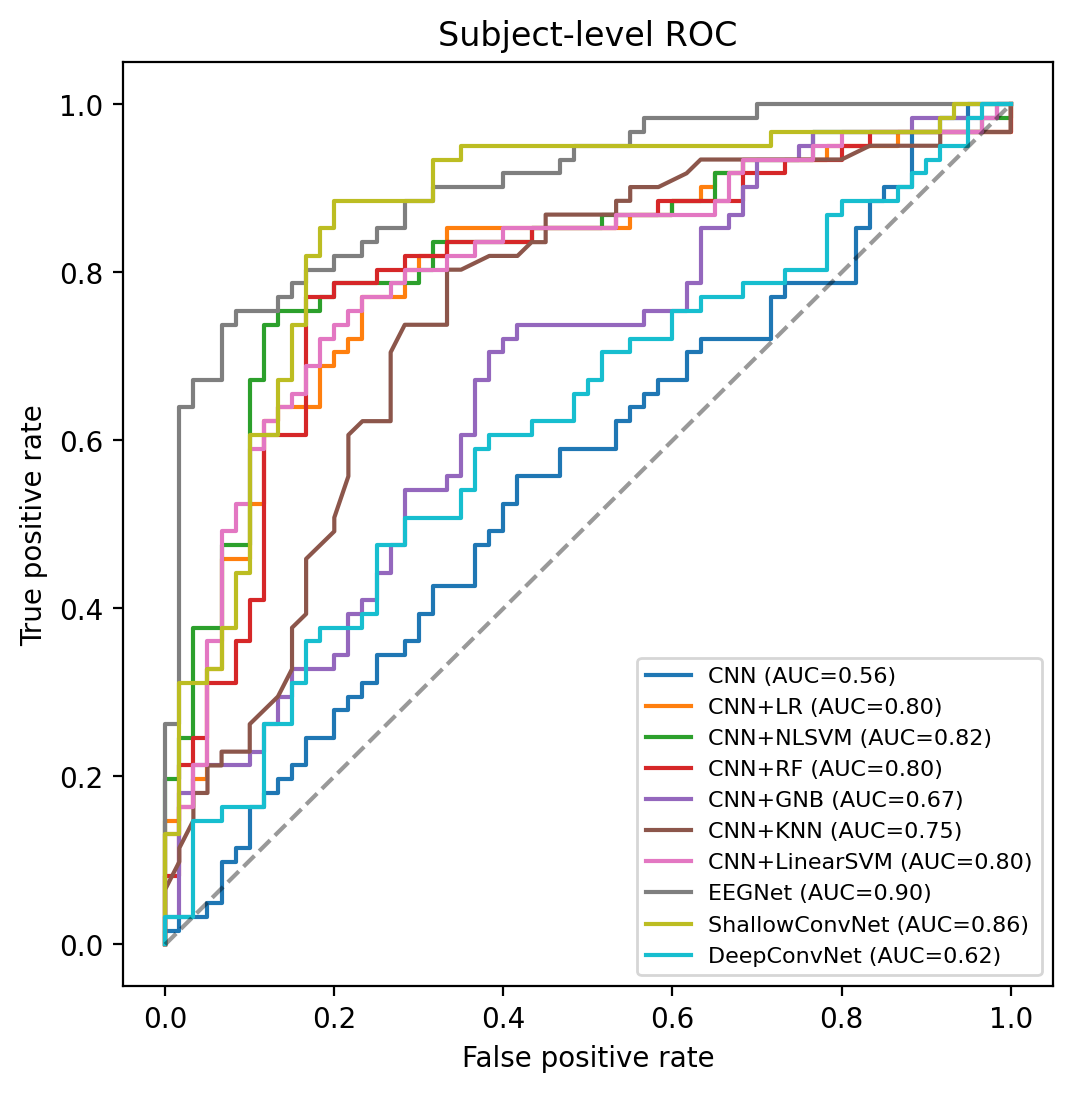
\includegraphics[width=\textwidth]{FIGURES/fig5_subject_roc.png}

\caption{Subject-level receiver operating characteristic (ROC) curves for all ten models, computed from the mean-predicted-probability aggregation described in Section 3.14 (n = 121 subjects each). Area-under-curve (AUC) values shown in the legend correspond to the AUC column of Table 3. EEGNet (AUC = 0.90) and ShallowConvNet (AUC = 0.86) dominate the other models across most of the false-positive-rate range; the plain CNN (AUC = 0.56) lies close to the chance diagonal.}

\label{fig:2}

\end{figure}

\begin{figure}[htbp]

\centering

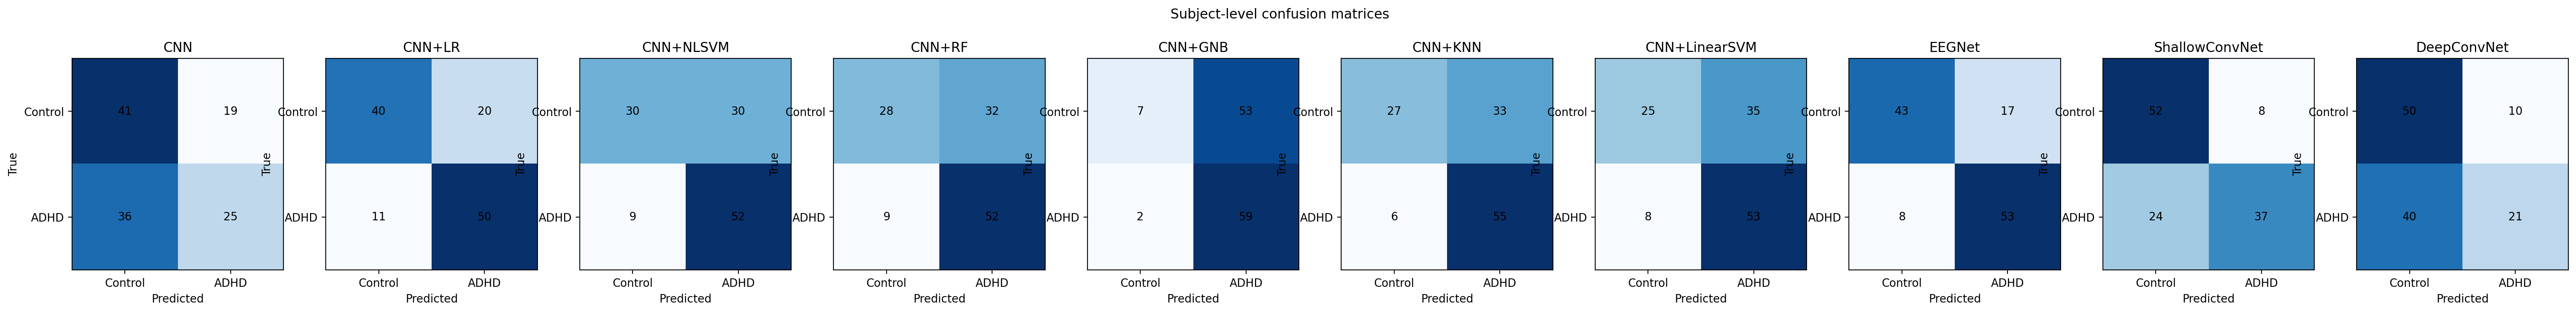
\includegraphics[width=\textwidth]{FIGURES/fig6_confusion.png}

\caption{Subject-level confusion matrices for all ten models (n = 121 subjects; Control = typically developing, ADHD = attention-deficit/hyperactivity disorder). Counts reproduce the sensitivity and specificity values reported in Table 3 -- for example, EEGNet's 43 true-negative and 53 true-positive counts correspond to its specificity of 0.717 and sensitivity of 0.869, and CNN+GNB's 59 true-positive versus 7 true-negative counts illustrate the strong bias toward the ADHD class discussed above.}

\label{fig:3}

\end{figure}

\subsection{Comparison with EEGNet, ShallowConvNet and DeepConvNet}

The three established EEG architectures diverge considerably from one another under this identical evaluation protocol. EEGNet outperforms the plain CNN by a wide margin (balanced accuracy 0.793 versus 0.547) and outperforms every CNN-derived hybrid classifier as well. ShallowConvNet reaches a balanced accuracy (0.737) comparable to the best-performing hybrid classifiers, but with a markedly different sensitivity/specificity balance (0.607/0.867) than EEGNet's (0.869/0.717) or the CNN-derived hybrids' (typically higher sensitivity than specificity), suggesting these architectures are not simply scaled versions of one another in terms of the decision boundary they learn, even though they are evaluated on identical folds. DeepConvNet, the deepest of the three architectures tested, performs no better than the plain CNN (Section 4.5), which is consistent with the possibility that its greater parameter count is not well matched to a dataset of this size (121 subjects, 508 epochs) without additional regularization or data beyond what was used here --- a possibility we return to in Section 5.4 without treating it as established, since parameter count is only one of several architectural differences between DeepConvNet and the better-performing models.



\subsection{Performance variability and confidence intervals}

Table 4 reports subject-level bootstrap 95\% confidence intervals (2000 resamples) for balanced accuracy and AUC for every model at 128 Hz, computed as described in Section 3.16.



\begin{table}[htbp]
\centering
\small
\caption{Table 4. Subject-level 95\% bootstrap confidence intervals, 128 Hz condition (selected metrics; full 8-metric table for both preprocessing conditions in the source file).}
\begin{tabular}{lll}
\toprule
Model & Balanced Acc. (95\% CI) & AUC (95\% CI) \\
\midrule
EEGNet & 0.793 (0.723--0.862) & 0.902 (0.844--0.949) \\
CNN+LR & 0.743 (0.662--0.819) & 0.800 (0.713--0.880) \\
ShallowConvNet & 0.737 (0.660--0.811) & 0.863 (0.791--0.927) \\
CNN+LR\_withCORAL & 0.735 (0.651--0.816) & 0.798 (0.708--0.876) \\
CNN+NLSVM & 0.676 (0.596--0.752) & 0.822 (0.739--0.896) \\
CNN+KNN & 0.676 (0.602--0.749) & 0.749 (0.657--0.836) \\
CNN+RF & 0.660 (0.580--0.739) & 0.797 (0.707--0.878) \\
CNN+LinearSVM & 0.643 (0.567--0.721) & 0.805 (0.719--0.883) \\
DeepConvNet & 0.589 (0.511--0.663) & 0.615 (0.507--0.719) \\
CNN & 0.547 (0.459--0.627) & 0.557 (0.457--0.660) \\
CNN+GNB & 0.542 (0.496--0.588) & 0.673 (0.574--0.765) \\
\bottomrule
\end{tabular}
\end{table}

\textit{Source: TABLE\_4\_CONFIDENCE\_INTERVALS.csv (160 rows total: 20 model$\times$preprocessing groups $\times$ 8 metrics). The full interval for every model and every metric (accuracy, balanced accuracy, sensitivity, specificity, precision, F1, MCC, AUC), at both preprocessing conditions, is available in the accompanying TABLES/ directory.}



The confidence intervals in Table 4 are wide relative to the point-estimate differences between several neighbouring models --- for example, ShallowConvNet's balanced-accuracy interval (0.660--0.811) and CNN+LR's (0.667--0.816) overlap substantially --- which is expected given the modest sample size (121 subjects) and is precisely the kind of uncertainty that a single point estimate, of the kind more commonly reported in the literature reviewed in Section 2, would obscure entirely.



Figure 4 shows these balanced-accuracy point estimates and 95\% confidence intervals for all ten models side by side, visually confirming the overlap described above.



\begin{figure}[htbp]

\centering

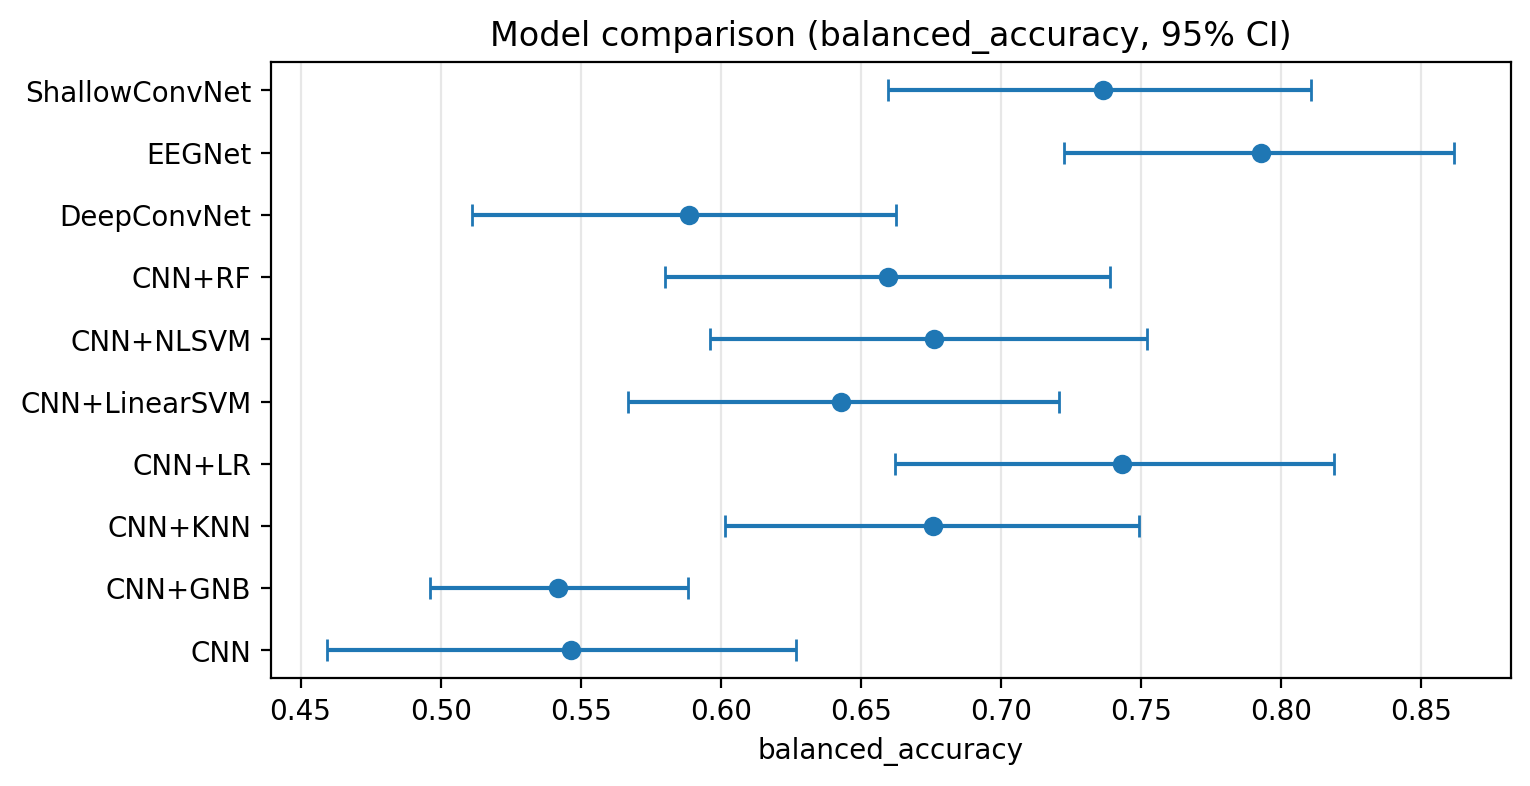
\includegraphics[width=\textwidth]{FIGURES/fig4_model_comparison_balanced_accuracy.png}

\caption{Subject-level balanced accuracy with 95\% bootstrap confidence intervals (2000 resamples) for all ten models at the native 128 Hz condition, corresponding to Table 4. EEGNet and ShallowConvNet's intervals lie clearly above DeepConvNet's and the plain CNN's, while the CNN-derived hybrid classifiers (CNN+LR, CNN+NLSVM, CNN+KNN, CNN+RF, CNN+LinearSVM) occupy an intermediate range with substantial mutual interval overlap.}

\label{fig:4}

\end{figure}

\subsection{Statistical comparison between models}

Table 5 reports the pre-specified subject-level paired comparisons against the plain CNN at 128 Hz as the reference model (Section 3.17): one paired observation per subject (n = 121), a paired bootstrap and a paired permutation test, both Holm-corrected within this 11-comparison family.



\begin{table}[htbp]
\centering
\small
\caption{Table 5. Subject-level paired balanced-accuracy comparisons against CNN|128 Hz (n = 121 subjects; paired bootstrap and paired permutation test, Holm-corrected).}
\begin{tabular}{lllll}
\toprule
Comparison & Mean diff. & 95\% CI of diff. & p (bootstrap, Holm) & p (permutation, Holm) \\
\midrule
CNN vs. EEGNet & +0.246 & (0.126, 0.362) & <0.0001 & 0.0016 \\
CNN vs. CNN+LR & +0.197 & (0.080, 0.308) & 0.0110 & 0.0185 \\
CNN vs. CNN+LR\_noCORAL & +0.197 & (0.080, 0.308) & 0.0110 & 0.0185 \\
CNN vs. ShallowConvNet & +0.190 & (0.075, 0.303) & 0.0110 & 0.0140 \\
CNN vs. CNN+LR\_withCORAL & +0.188 & (0.068, 0.304) & 0.0133 & 0.0242 \\
CNN vs. CNN+KNN & +0.129 & (0.018, 0.236) & 0.1284 & 0.3240 \\
CNN vs. CNN+NLSVM & +0.130 & (0.016, 0.239) & 0.1284 & 0.3240 \\
CNN vs. CNN+RF & +0.113 & (-0.001, 0.224) & 0.2080 & 0.3876 \\
CNN vs. CNN+LinearSVM & +0.096 & (-0.019, 0.209) & 0.3021 & 0.5253 \\
CNN vs. DeepConvNet & +0.042 & (-0.069, 0.150) & 0.9082 & 0.7734 \\
CNN vs. CNN+GNB & -0.005 & (-0.096, 0.083) & 0.9085 & 0.9023 \\
\bottomrule
\end{tabular}
\end{table}

\textit{Source: TABLE\_5\_MODEL\_COMPARISON\_STATISTICS.csv, generated by \texttt{src/subject\_level\_paired\_test.py} from \texttt{results\_final/predictions/all\_predictions.csv} (20,000 bootstrap resamples, 20,000 permutations, seed 12345). Mean diff. and CI are from the bootstrap distribution.}



After Holm correction, four comparisons remain statistically significant by both the bootstrap and the permutation test: EEGNet, ShallowConvNet, and the CNN-plus-logistic-regression classifier in both its CORAL configurations (CNN+LR/CNN+LR\_noCORAL and CNN+LR\_withCORAL are numerically identical to each other, as noted in Section 3.18, so these two rows reflect one classifier evaluated with and without CORAL alignment rather than two independent classifiers). Counting distinct classifiers rather than table rows, three configurations show a confirmed advantage over the plain CNN --- EEGNet, ShallowConvNet, and CNN+LR (with or without CORAL) --- while CNN+KNN, CNN+NLSVM, CNN+RF, CNN+LinearSVM, DeepConvNet, and CNN+GNB do \textbf{not} reach significance after correction under this subject-level test, despite several of them (KNN, NLSVM, RF) having reached nominal significance under the repeated-fold Wilcoxon procedure described in Section 3.17 --- a direct illustration of why that procedure was not retained as the primary test. We report this as a genuine, and in part negative, finding: only EEGNet, ShallowConvNet, and the CNN+LR configuration show a subject-level balanced-accuracy advantage over the plain CNN that survives a statistically defensible test and multiplicity correction; the apparent advantage of the remaining hybrid classifiers over the plain CNN, while numerically present in Table 3, is not distinguishable from sampling variability at this sample size (n = 121 subjects) once fold-level pseudo-replication is removed. DeepConvNet does not differ significantly from the plain CNN under either test (bootstrap p = 0.908; mean difference +0.042, the smallest positive difference of any comparison in this table other than CNN+GNB's negative one).



Figure 5 shows the distribution of balanced accuracy across the 25 per-(repetition, outer-fold) estimates for each model, at the native 128 Hz condition. This distribution is reported descriptively, to illustrate fold-to-fold variability under repeated cross-validation; because the underlying 121 subjects are reused across repetitions (Section 3.17), the 25 points per model are not treated as 25 independent observations, and are not the basis of the significance tests reported in Table 5.



\begin{figure}[htbp]

\centering

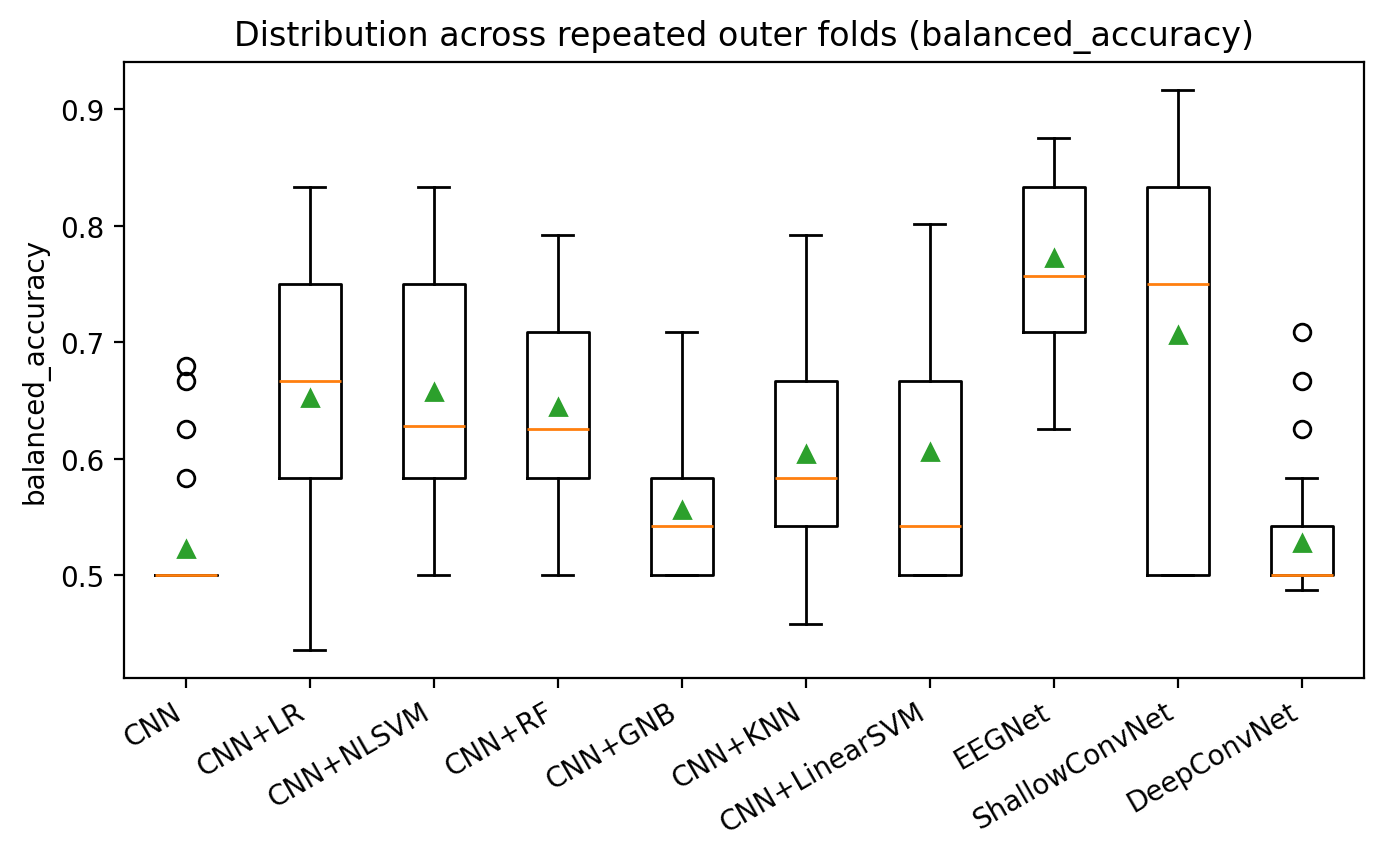
\includegraphics[width=\textwidth]{FIGURES/fig7_repeated_cv_distribution_balanced_accuracy.png}

\caption{Distribution of balanced accuracy across the 25 per-(repetition, outer-fold) estimates (5 outer folds x 5 repetitions; Section 3.13) for each model, at the native 128 Hz condition, shown descriptively to illustrate fold-to-fold variability. Boxes show the interquartile range and median (orange line); green triangles mark the mean. Because these 25 estimates per model reuse the same 121 subjects across repetitions, they are not independent observations and are not the basis of Table 5's subject-level significance tests (Section 3.17); the wide spread shown here nonetheless illustrates why a single held-out point estimate would be an unreliable summary of any one model's performance.}

\label{fig:5}

\end{figure}

\subsection{CORAL domain-adaptation analysis}

CORAL-aligned features (CNN+LR\_withCORAL, balanced accuracy 0.735, 95\% CI 0.651--0.816) did not outperform the unaligned features (CNN+LR / CNN+LR\_noCORAL, balanced accuracy 0.743, 95\% CI 0.662--0.819); the point estimate is marginally lower with alignment applied, and the two intervals overlap almost completely. We did not run a dedicated paired significance test between these two specific configurations (Table 5's reference model is the plain CNN, not CNN+LR\_noCORAL), so this should be read as an observed, not a statistically confirmed, difference. Figure 6 shows the covariance-distance reduction achieved by CORAL alignment (left panel) alongside the resulting per-outer-fold accuracy distributions with and without alignment (right panel): the covariance distance between outer-train and outer-test feature distributions drops sharply and consistently after alignment, confirming the alignment step itself worked as intended, while the downstream accuracy distributions remain essentially overlapping --- the mechanism did what it was designed to do without translating into a detectable classification benefit in this setting, a dissociation discussed further in Section 5.7.



\begin{figure}[htbp]

\centering

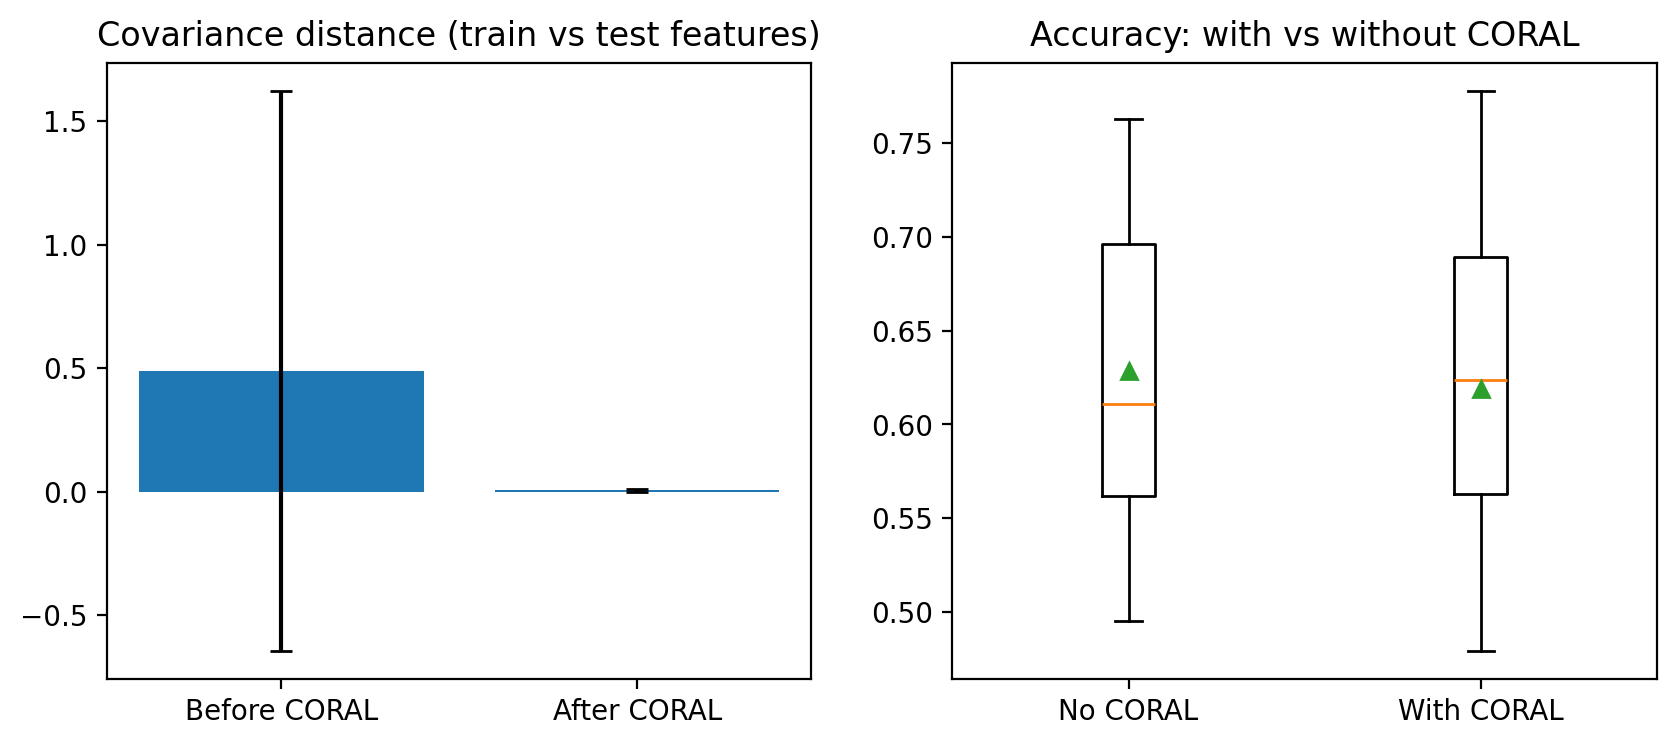
\includegraphics[width=\textwidth]{FIGURES/fig10_coral_covariance.png}

\caption{CORAL domain adaptation. Left: covariance distance (Frobenius norm) between outer-train and outer-test CNN feature distributions before and after CORAL alignment, pooled across all outer folds and repetitions -- alignment reduces this distance sharply and consistently. Right: per-outer-fold epoch-level accuracy of the downstream logistic-regression classifier without versus with CORAL alignment, showing near-identical distributions despite the large reduction in covariance distance on the left.}

\label{fig:6}

\end{figure}

\subsection{Resolution sensitivity analysis}

Table 6 reports the 128 Hz-versus-128-to-512-Hz-interpolation comparison for CNN and EEGNet (Section 3.19).



\begin{table}[htbp]
\centering
\small
\caption{Table 6. Resolution sensitivity analysis (subject-level, n = 121 subjects; paired test uses 5 outer folds from a single shared repetition).}
\begin{tabular}{lllll}
\toprule
Model & Preprocessing & Accuracy & Balanced Acc. & AUC \\
\midrule
CNN & 128 Hz & 0.545 & 0.547 & 0.557 \\
CNN & 128-to-512 Hz interp. & 0.587 & 0.586 & 0.631 \\
EEGNet & 128 Hz & 0.793 & 0.793 & 0.902 \\
EEGNet & 128-to-512 Hz interp. & 0.736 & 0.735 & 0.846 \\
\bottomrule
\end{tabular}
\end{table}

\textit{Paired test (balanced accuracy, Holm-corrected within this 2-comparison family):}



\begin{table}[htbp]
\centering
\small
\begin{tabular}{lllll}
\toprule
Comparison & n paired folds & Mean diff. & 95\% CI of diff. & p-value \\
\midrule
CNN: 128 Hz vs. interp. & 5 & -0.067 & (-0.195, 0.061) & 0.50 \\
EEGNet: 128 Hz vs. interp. & 5 & +0.049 & (0.0006, 0.098) & 0.19 \\
\bottomrule
\end{tabular}
\end{table}

\textit{Source: TABLE\_6\_128HZ\_VS\_128TO512.csv, TABLE\_6\_128HZ\_VS\_128TO512\_paired\_test.csv.}



Neither comparison reaches significance at $\alpha$ = 0.05. For CNN, the interpolated condition scores numerically higher (0.586 versus 0.547); for EEGNet, the native condition scores numerically higher (0.793 versus 0.735); neither direction is statistically supported given only 5 paired outer folds, and we do not interpret either numerical difference as evidence that interpolation helps or harms classification, nor as evidence about the original recording's true sampling rate (Section 5.6).



Figure 7 shows the full distribution underlying these comparisons for CNN (panel a) and EEGNet (panel b) separately.



\begin{figure}[htbp]

\centering

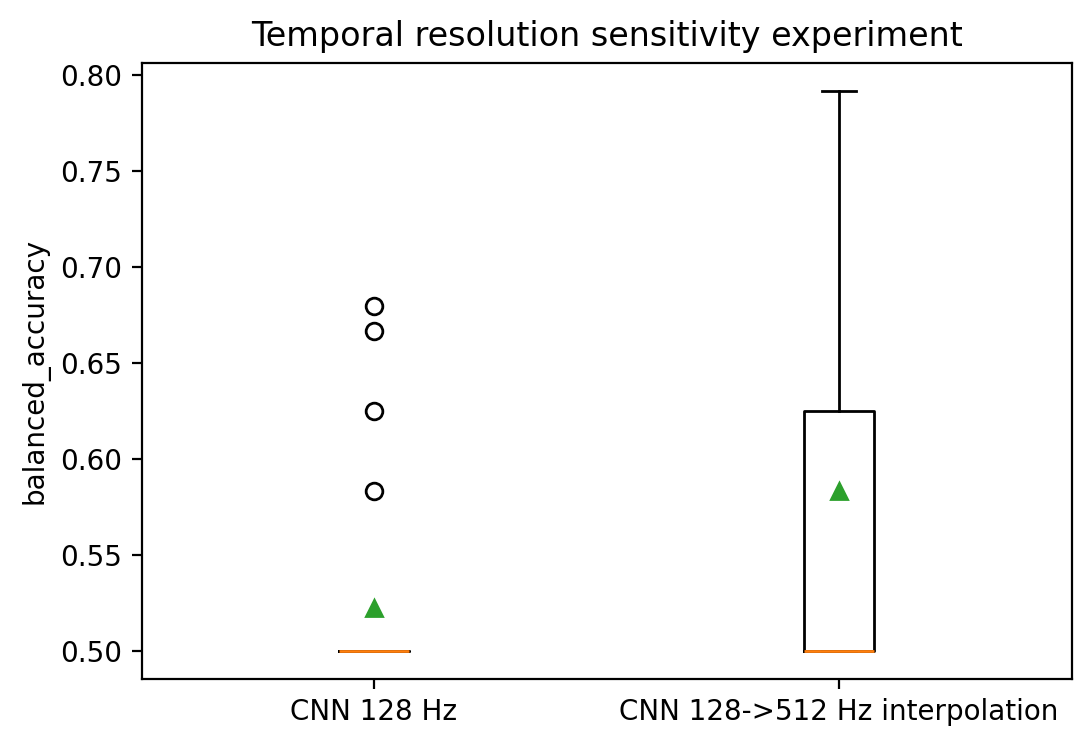
\includegraphics[width=\textwidth]{FIGURES/fig8_resolution.png}

\caption{Distribution of balanced accuracy across the 5 paired outer folds for the CNN model, native 128 Hz versus 128-to-512 Hz FFT-interpolated condition. Open circles mark individual fold values (n = 5 per condition, too few to resolve as a conventional box in the 128 Hz condition); the green triangle marks the mean.}

\label{fig:7a}

\end{figure}

\begin{figure}[htbp]

\centering

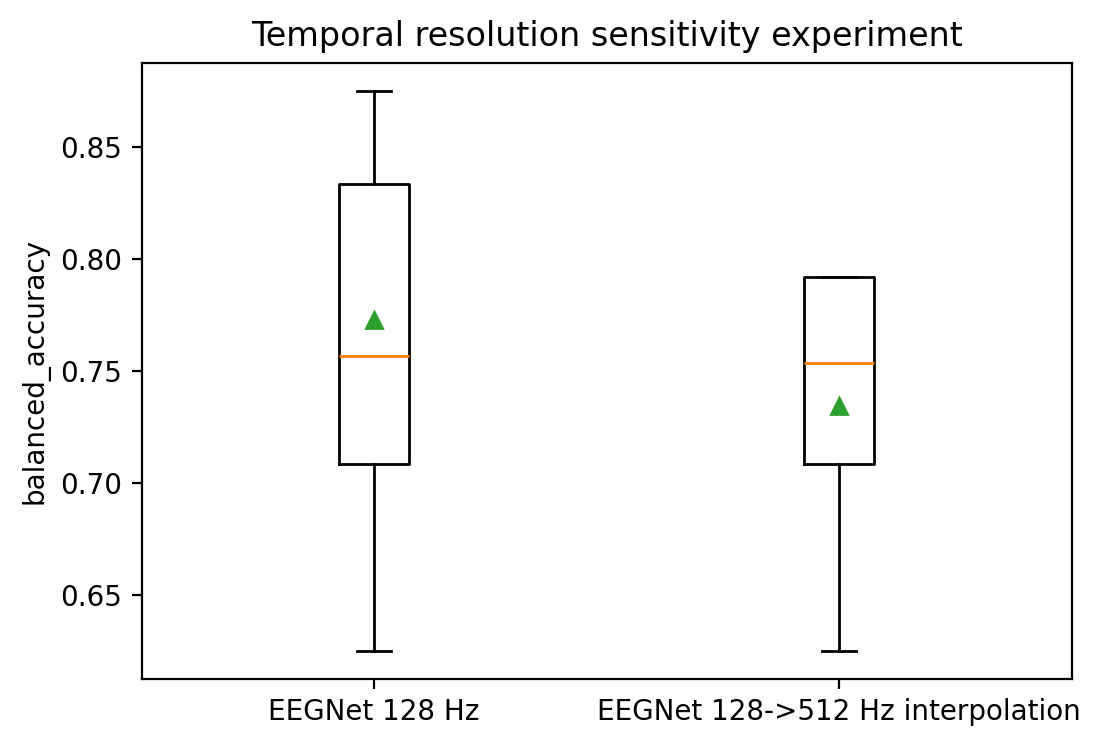
\includegraphics[width=\textwidth]{FIGURES/fig8_resolution_EEGNet.png}

\caption{Distribution of balanced accuracy across the 5 paired outer folds for the EEGNet model, native 128 Hz versus 128-to-512 Hz FFT-interpolated condition, plotted on the same scale convention as panel a.}

\label{fig:7b}

\end{figure}

\section{Discussion}

\subsection{Principal findings}

Under a nested, repeated, subject-independent evaluation design, the raw-EEG CNN architecture used in the original study we reassess here performs close to chance at the subject level (balanced accuracy 0.547), while several classical classifiers trained on that same CNN's extracted features, and two of three established EEG deep-learning architectures tested alongside it, achieve numerically higher balanced accuracy. Under a subject-level paired statistical test (Section 3.17), however, only three of these configurations --- EEGNet, ShallowConvNet, and the CNN-plus-logistic-regression classifier --- show an advantage over the plain CNN that survives correction for multiple comparisons; the remaining hybrid classifiers' higher point estimates, and DeepConvNet's, are not statistically distinguishable from sampling variability at this sample size. This pattern --- a weak base architecture rescued by a downstream classical classifier in at least one case, matched or exceeded by an architecture (EEGNet) designed specifically for EEG rather than borrowed from a generic image-classification convolutional template, and only partially confirmed once repeated-fold pseudo-replication is removed from the significance test --- is, to our reading, the central empirical finding of this study, more informative than any single headline accuracy number taken in isolation.



\subsection{Effect of subject-independent validation}

We did not run the original grouped-ten-fold protocol from \cite{taghibeyglou2022detection} ourselves on this codebase, so we cannot report a direct, matched before/after comparison of leakage-permitting versus leakage-controlled validation on identical code. What we can say is that our epoch-level, pooled results (Table 2) --- themselves computed under the same nested, subject-independent partition, simply aggregated differently --- fall in a broadly comparable range to the original study's reported grouped-cross-validation figures for several models, while our subject-level figures diverge from any single epoch-level number by an amount that depends heavily on which classifier is examined (compare, for the plain CNN, an epoch-level balanced accuracy of 0.516 against a subject-level balanced accuracy of 0.547 --- a small difference in this specific case --- against EEGNet's epoch-level 0.765 versus subject-level 0.793, again a modest difference). Because both the epoch-level and subject-level results reported here use subject-grouped partitions, their difference cannot be used to quantify the effect of subject leakage. A direct estimate would require a separate segment-level evaluation allowing same-subject epochs to cross the train/test boundary, which is outside the scope of what this study set out to measure.



\subsection{CNN versus classical hybrid classifiers}

The gap between the plain CNN (balanced accuracy 0.547) and the same CNN's features routed through logistic regression (0.743, a statistically significant advantage under the subject-level test in Section 4.6) is consistent with the CNN's own final dense-and-sigmoid classification head not extracting all of the discriminative information present in its own penultimate-layer representation --- since a linear classifier fit on that exact representation recovers more of it. The other CNN-derived classical classifiers (e.g. an RBF support vector machine, balanced accuracy 0.676) show a numerically similar pattern, though their individual advantage over the plain CNN did not reach significance after correction (Section 4.6), so this explanation is best treated as most directly supported by the logistic-regression comparison specifically. A plausible explanation, which this study's design cannot fully adjudicate, is that the CNN's small dataset (Section 6) makes its jointly trained classification head prone to a degree of overfitting or under-optimization that a separately fit, appropriately regularized classical classifier is less susceptible to on the same fixed features. The comparatively poor performance of CNN+GNB and the extreme sensitivity/specificity imbalance it exhibits (0.967/0.117) is most parsimoniously explained by its lack of a class-weighting mechanism (Section 3.8) combined with the fixed feature representation not being especially well suited to Gaussian naive Bayes's conditional-independence assumption, rather than by any property of the CNN features specific to this comparison.



\subsection{EEGNet, ShallowConvNet, and DeepConvNet comparison}

EEGNet's advantage over the plain CNN, ShallowConvNet, and DeepConvNet in this study is consistent with EEGNet's design intent: its depthwise-and-separable convolutional structure was built specifically to encode standard EEG feature-extraction concepts (spatial filtering, followed by temporal filtering per spatial filter) with a parameter-efficient architecture, whereas the CNN evaluated here uses a more generic two-stage spatial-then-temporal convolutional design not specifically tailored to EEG, and DeepConvNet's substantially larger parameter count is a plausible, though not confirmed, contributor to its comparatively weak generalization on a dataset of only 121 subjects. ShallowConvNet's markedly different sensitivity/specificity balance relative to EEGNet, despite a similar balanced-accuracy point estimate, is worth noting for any future clinical framing of these results: two models can appear similarly "accurate" in balanced-accuracy terms while making very different kinds of errors, and which error profile is preferable depends on the clinical context in which such a tool might eventually be used, a question this study does not address.



\subsection{Importance of subject-level evaluation}

The consistent practice, throughout Section 4, of reporting subject-level results as primary and epoch-level results as a clearly labelled secondary quantity reflects a methodological position, not merely a presentational choice: 508 epochs distributed unevenly across 121 children do not constitute 508 independent trials of an underlying diagnostic test, and treating them as such --- as a pooled epoch-level table implicitly does --- both overstates the effective sample size available for computing performance and can systematically favor a classifier that happens to perform particularly well or poorly on the specific subjects who contribute unusually many epochs. Every comparison and every confidence interval in Section 4 that this paper treats as a primary result is computed at the subject level for exactly this reason.



\subsection{Resolution sensitivity}

The absence of a statistically significant difference between the native 128 Hz and the 128-to-512 Hz interpolated representation, for both CNN and EEGNet, should be read narrowly: it indicates that this specific FFT-interpolation procedure, applied to this specific dataset and these two architectures, did not produce a detectable change in subject-level balanced accuracy at the sample size available (5 paired outer folds). It does not indicate, and should not be cited as indicating, anything about whether the released files were originally recorded at 128 Hz, at 512 Hz, or at some other rate; interpolation cannot recover information that was not present in the samples being interpolated, so a null result here is fully consistent with the recording having been made at either rate, or with the CNN and EEGNet architectures evaluated here simply not being sensitive to whatever difference interpolation does or does not introduce. We report this analysis to close off resolution as an unaddressed confound, not to make a claim about the dataset's true acquisition parameters.



\subsection{CORAL and cross-subject domain adaptation}

That CORAL alignment did not improve, and if anything marginally reduced, the logistic-regression classifier's balanced accuracy in this study is itself an informative negative result given how frequently correlation alignment and its variants are reported as beneficial in the broader EEG domain-adaptation literature \cite{li2026crosssubject,zhong2023deep}. One plausible interpretation is that the outer-training and outer-test feature covariances, both drawn from the same CNN trained on the same task and the same broad population (children recruited under one study protocol), may already be similar enough that covariance alignment has little further shift to correct, in contrast to cross-session or cross-device transfer settings where CORAL and its relatives were originally shown to help. We did not test CORAL under a setting with a more deliberately induced distribution shift (e.g., across recording sites or acquisition sessions), and we would regard that as a more informative test of this specific hypothesis than anything this study's design can offer on its own.



\subsection{Relationship to previously reported ADHD-EEG performance}

The comparison that motivated this study most directly --- Amini et al.'s ADHDeepNet \cite{amini2025adhdeepnet}, evaluated by the authors' own description with nested cross-validation on what appears to be the same 121-participant dataset used here, reporting 99.17\% accuracy and 100\% sensitivity --- sits far outside the 0.55--0.79 balanced-accuracy range obtained across every model tested in the present study, including EEGNet, the best performer here. We are not in a position to identify the specific source of this gap without access to that study's training code, fold-assignment logs, and exact aggregation procedure, and we explicitly decline to assert that their reported nested cross-validation contains subject leakage; it may not. What we can say, on the basis of the evidence gathered here, is that a carefully audited nested, subject-independent, subject-level evaluation of a broadly comparable CNN-based pipeline on the same underlying population does not reproduce anything close to that figure for any architecture tested, including ones (EEGNet) considerably more parameter-efficient and EEG-specific than a plain CNN. The same observation applies, with somewhat less certainty about dataset overlap, to Hassan and Singhal's reported 100\% accuracy, sensitivity, and specificity using a similarly structured 19-channel CNN pipeline \cite{hassan2024convolutional}. Two properties any reader should check before accepting a near-ceiling EEG classification result at face value, and which we recommend future ADHD-EEG papers state explicitly, are: (i) whether the accuracy is computed per epoch or per subject, and (ii) whether every subject's epochs were confined to a single side of the train/test boundary in every fold used to compute that reported number, including any fold used for early stopping or hyperparameter selection.



\subsection{Methodological implications}

Beyond the specific numbers reported here, the largest methodological implication of this study is that a single validation protocol is not sufficient to characterize an EEG classification pipeline's real-world generalization: the outer-loop-only pooled accuracy, the nested subject-level accuracy, and the confidence interval around that subject-level accuracy each answer a different question, and a manuscript reporting only the first of these three quantities leaves a reader unable to judge how much of the reported performance would survive a more conservative evaluation, or how much sampling variability that performance figure actually carries.



\subsection{Practical and clinical implications}

No model evaluated in this study reaches a level of subject-level performance (balanced accuracy 0.79 at best, for EEGNet) that we would characterize as clinically actionable in isolation, whether framed as a diagnostic aid, a screening tool, or any other decision-support role; EEG-based classification of this kind is, at the current stage of evidence represented by this study and the wider literature reviewed in Section 2, a research finding about population-level separability of two groups under a controlled task, not a validated instrument for individual clinical decision-making. Any future work aimed at a practical application would additionally require external validation on data collected at a different site, under different recording equipment, and ideally with a prospective rather than retrospective design, none of which this study attempts or claims to provide.



We now turn to the limitations of the present study explicitly, in Section 6, before concluding in Section 7.



\section{Limitations}

This study has a number of limitations that bear directly on how its results should be interpreted and generalized.



\textbf{Sample size.} The dataset comprises 121 subjects, which is modest by the standards of deep-learning classification generally, though not atypical for clinical EEG studies in a pediatric population where recruitment is inherently constrained. The wide bootstrap confidence intervals reported in Table 4 (e.g., a roughly 15-percentage-point-wide interval for several models' balanced accuracy) are a direct, honestly reported consequence of this sample size, not an artifact of the bootstrap procedure itself.



\textbf{Single public dataset, single site.} All results in this study come from one dataset, collected at one recording site, under one task protocol. No claim is made, or should be inferred, about how any of these models would perform on EEG collected with different equipment, a different task, a different age range, or a different clinical population.



\textbf{No external validation.} This study performs internal, albeit rigorously subject-independent, cross-validation; it does not include a prospectively collected or externally sourced validation cohort. Internal cross-validation, however carefully controlled, estimates how well a model would generalize to \textit{new subjects drawn from the same recording protocol and population}, not to a genuinely external population.



\textbf{Sampling-rate metadata limitation.} As discussed throughout Sections 3.1, 3.19, 4.8, and 5.6, the true sampling rate of the released recordings could not be independently verified, and the 128 Hz assumption --- used identically in the original study this paper reassesses --- remains an assumption rather than a confirmed fact.



\textbf{Interpolation is not equivalent to genuine higher-rate acquisition.} The 128-to-512 Hz condition tested in this study is FFT interpolation of the existing 128 Hz samples and must not be read, here or in any future citation of this work, as equivalent to, or a stand-in for, a genuine 512 Hz recording.



\textbf{Architecture-fidelity caveat.} EEGNet, ShallowConvNet, and DeepConvNet were reimplemented from their published architecture descriptions \cite{lawhern2018eegnet,schirrmeister2017deep} rather than imported from an externally maintained, independently verified implementation, and we did not undertake a line-by-line verification of our implementation against the original authors' own code. We consider this an acceptable basis for the comparative claims made in this study, since all three architectures were implemented, trained, and evaluated under exactly the same protocol and by the same authors, but a reader intending to cite specific numeric performance figures as a faithful reproduction of the original EEGNet or ShallowConvNet/DeepConvNet papers should treat this reimplementation as an independent variable worth checking.



\textbf{CORAL and Integrated Gradients implementation provenance.} The CORAL alignment procedure and the Integrated Gradients attribution procedure used in this study were each implemented from the general mechanics described in their respective source papers \cite{sun2016return,sundararajan2017axiomatic} rather than from a fresh, formula-by-formula re-derivation immediately before this study began; we consider the resulting implementations mechanically correct (their outputs behave as expected --- e.g., CORAL reduces the measured covariance distance between source and target features, and Integrated Gradients attributions sum, as they should by construction, to the difference between the model's output at the actual input and at the baseline), but recommend this same caveat to any reader planning to cite the exact numerical CORAL or Integrated Gradients formulation as verified against the original publications independently of this study.



\textbf{GPU nondeterminism.} As noted in Section 3.13, a small amount of run-to-run variability from non-deterministic GPU convolution kernels is possible even with fixed random seeds; this is a documented property of the deep-learning framework used, not specific to this study's implementation, and CPU execution under the same seeds is fully deterministic.



\textbf{Correlation among repeated-CV estimates.} The 25 per-(repetition, outer-fold) balanced-accuracy values produced by the repeated-CV design (5 repetitions $\times$ 5 outer folds) reuse the same 121 subjects across repetitions and are therefore correlated, not independent; Section 3.17 explains why the primary model comparisons in Table 5 use a subject-level paired bootstrap and permutation test (one observation per subject, n = 121) rather than treating these 25 values as independent replicates. Figure 5 still reports the repeated-fold distribution, but descriptively, to show fold-to-fold variability, not as the basis for inference.



\textbf{Limitations of the inferential procedure itself.} The subject-level bootstrap and permutation tests used here assume the 121 subjects are themselves a representative, independently sampled cohort from the population the study intends to generalize to; violations of that assumption (e.g., unmeasured site- or recruitment-related clustering within the dataset) would not be detected by either test. Both tests are also comparisons of point predictions (thresholded at 0.5) rather than of the full predicted-probability distributions, and neither test can distinguish a true absence of a population-level difference from a difference too small to detect at n = 121.



\textbf{Transductive nature of CORAL.} As stated in Section 3.18, the CORAL analysis (CNN+LR\_withCORAL) computes its target covariance from the outer-test subjects' own unlabelled features before evaluating on those same subjects; this is a transductive, unsupervised domain-adaptation setting, not the fully inductive subject-independent evaluation used for every other model in this study, and the two should not be read as subject to identical generalization guarantees.



\textbf{Limited scope of the resolution-sensitivity experiment.} The 128-to-512 Hz interpolation comparison (Section 3.19, Section 4.8) was run for only two architectures (the plain CNN and EEGNet), using a single repetition (5 outer folds, not the full repeated design), and using one specific interpolation procedure (FFT-based polyphase resampling). Its null result should not be extrapolated to the other nine models evaluated in this study, to a different interpolation method, or beyond the specific comparison tested.



\textbf{Model-dependent and dataset-specific results.} The relative ranking of models reported here (EEGNet best, plain CNN and DeepConvNet weakest, classical hybrid classifiers in between) should not be assumed to generalize to a different EEG-based classification task, a different age range, or a different clinical population without separate evaluation.



\textbf{No prospective or clinical-utility evaluation.} This study does not evaluate, and makes no claim about, clinical utility, cost-effectiveness, or real-world diagnostic added value beyond existing behavioural assessment; such claims would require a substantially different, prospective study design.



\textbf{Ablation study not included in this manuscript.} The codebase underlying this study includes an architectural ablation framework (varying the presence of spatial convolution, temporal convolution, batch normalization, and pooling within the CNN), but ablation results were not part of the final combined result set used to produce Section 4 and are therefore not reported here; we note this explicitly rather than omitting mention of the capability, so that a reader consulting the accompanying repository is not surprised to find ablation-related code with no corresponding results in this manuscript.



\section{Conclusion}

This study set out to determine how much of a previously reported raw-EEG CNN-and-hybrid-classifier pipeline's classification performance for ADHD survives a genuinely subject-independent, nested, repeated evaluation with subject-level aggregation, a statistically defensible subject-level comparison procedure, and explicit uncertainty quantification, and to compare that pipeline against established EEG deep-learning architectures under the same protocol. The answer, on this dataset, is that performance survives only partially and unevenly: the original plain CNN performs close to chance at the subject level (balanced accuracy 0.547); one classical classifier trained on that CNN's own extracted features, logistic regression, recovers substantially more discriminative signal (0.743) and does so with a subject-level paired advantage over the plain CNN that survives correction for multiple comparisons, while the remaining classical classifiers show a numerically higher but not statistically confirmed advantage; and EEGNet and ShallowConvNet --- architectures designed specifically for EEG rather than adapted from a generic convolutional template --- both show a confirmed subject-level advantage over the plain CNN (balanced accuracy 0.793 and 0.737 respectively), with EEGNet outperforming every configuration tested here, while DeepConvNet shows a higher point estimate than the plain CNN (0.589 versus 0.547) but no statistically confirmed advantage. None of these figures approach the 95--100\% accuracies reported by several recent studies applying superficially similar CNN pipelines to the same or closely related data, a gap this study cannot fully explain without access to those studies' training code and fold assignments, but can characterize precisely on its own data and protocol. We take the central lesson of this study to be methodological rather than architectural: subject-level, uncertainty-quantified, nested-cross-validated evaluation, paired with a statistically defensible subject-level comparison procedure, is not an optional refinement for EEG-based ADHD classification research, but a precondition for any reported performance figure to be interpretable, comparable across studies, or eventually relevant to any downstream application --- clinical or otherwise.



\section*{Acknowledgements}
The EEG dataset analyzed in this study was collected and released by
TaghiBeyglou et al.; see the Data Availability statement below.

\section*{Data Availability}
The EEG dataset analyzed in this study is a publicly available dataset originally described by TaghiBeyglou et al. \cite{taghibeyglou2022detection}; it is not redistributed as part of this manuscript or its accompanying repository, consistent with the terms under which it is released. All analysis code, the leakage-audit implementation, the table- and figure-generation scripts, and the exact configuration used to produce the results in Section 4 are available at the repository and commit stated in Appendix~\ref{sec:appendix:repro}. The GitHub repository is cited here as the location of the code and generated artifacts underlying this manuscript; it is not cited as an independent source of scientific evidence, which rests on the dataset, the described methodology, and the result files it was used to produce.



\section*{Competing Interests}
The author declares no competing interests.

\section*{Funding}
The author received no specific funding for this work.

\section*{CRediT authorship contribution statement}
\textbf{Abinaya G:} Conceptualisation, Investigation, data curation,
methodology, software, formal analysis, validation, writing -- original
draft, writing -- review \& editing.

\section*{Ethical statement}
This study is a secondary, retrospective analysis of a previously collected, publicly released, de-identified EEG dataset \cite{taghibeyglou2022detection}. No new human-subjects data collection was performed for this study, and no new institutional ethical approval was sought or is claimed for this secondary analysis. Any ethical approval, consent procedure, or institutional review governing the original data collection is a matter of record in the original dataset's own documentation and the original publication \cite{taghibeyglou2022detection}, not restated or independently verified here.



\printcredits

\clearpage
\appendix
\section{Reproducibility Appendix}
\label{sec:appendix:repro}

\textbf{Original training run.}



\begin{itemize}

\item \textbf{Repository}: \texttt{https://github.com/abinaya-g/ADHD-EEG-Benchmark}

\item \textbf{Branch}: \texttt{claude/adhd-eeg-manuscript-revision-boeb24}

\item \textbf{Commit}: \texttt{6f0c1e8} (the commit that froze this manuscript revision together with \texttt{results\_final/predictions/all\_predictions.csv} and \texttt{manuscript/TABLES/})

\item \textbf{Dataset}: public Kaggle dataset associated with TaghiBeyglou et al. \cite{taghibeyglou2022detection} (121 subjects, 61 ADHD / 60 control, 19-channel EEG); not redistributed by this repository.

\item \textbf{Cross-validation design}: 5 outer folds, 4 inner folds, 5 repetitions, seeds [42, 43, 44, 45, 46] (each repetition's 5 outer folds use a fold-level seed derived from its repetition seed, e.g. 42000--42004 for repetition 42; see Section 3.12--3.13 and \texttt{results\_final/predictions/all\_predictions.csv}'s \texttt{seed} column).

\item \textbf{Training configuration}: Adam optimizer, learning rate $1\times10^{-4}$, batch size 16, maximum 100 training epochs, early-stopping patience 8 epochs (monitored on inner-validation loss); 2000 resamples for the subject-level bootstrap confidence intervals in Table 4.

\item \textbf{Software/hardware}: TensorFlow/Keras and scikit-learn, run on a cloud GPU instance (NVIDIA Tesla T4); CUDA/cuDNN versions not captured. The exact package version numbers (TensorFlow, scikit-learn, NumPy, SciPy, Python) actually used for this run were not recorded at run time; this project's dependency file pins \texttt{tensorflow==2.21.0}, but the run used a cloud notebook environment's preinstalled build rather than this pinned version, and the two are not confirmed identical. This is a genuine reproducibility gap, stated here rather than papered over with an unverified version number.

\item \textbf{Determinism}: CPU execution is deterministic under the stated seeds; GPU execution may show small run-to-run variation in some non-deterministic convolution kernels.

\end{itemize}

\textbf{Verification environment (this audit).} All numbers in Section 4 were independently re-derived from the raw prediction-level file \texttt{results\_final/predictions/all\_predictions.csv} (34,544 rows: one row per epoch $\times$ model $\times$ preprocessing-condition $\times$ repetition) using the environment below; this environment was used only to recompute metrics and run the statistical tests below from already-saved predictions, not to retrain any model.



\begin{itemize}

\item \textbf{Python}: 3.11.15

\item \textbf{TensorFlow}: 2.21.0 (CPU build; not used for training in this verification pass)

\item \textbf{Keras}: 3.15.1

\item \textbf{NumPy}: 2.4.6

\item \textbf{SciPy}: 1.17.1

\item \textbf{scikit-learn}: 1.9.0

\item \textbf{GPU / CUDA / cuDNN}: none available in this verification environment (CPU only)

\item Every value in Table 2 and Table 3 was independently recomputed from \texttt{all\_predictions.csv} and matched the corresponding table to within 1e-5; the subject-to-outer-fold partition was independently checked and confirmed to contain no cross-fold subject splits for any of the 12 models across all 5 repetitions (Section 4.2).

\item Table 5's subject-level paired bootstrap and permutation test (20,000 resamples / 20,000 permutations, seed 12345) was run with \texttt{src/subject\_level\_paired\_test.py}, included in the repository referenced above, reading directly from \texttt{all\_predictions.csv}.

\item All code, the automated 14-point leakage audit (\texttt{src/sanity\_checks.py}), the raw prediction file, and the table/figure-generation scripts used to produce every number in Section 4 are included in the repository referenced above.

\end{itemize}

\bibliographystyle{model1-num-names}
\bibliography{references}

\end{document}
